% ============================================================================
\section{Results}
\label{sec:results}

% ----------------------------------------------------------------------------
\subsection{Seizure simulation}

\paragraph{Models 1 and 2.} Weakening inhibition in the spiking network raised the synchrony index from 0.02 to 0.98, and restoring it brought the index back to 0.02 (Figure~\ref{fig:net}). The Epileptor produced 3 seizures in 6,000 time units at $x_0=-1.6$, with 51.6\% of the time ictal, and none at $x_0=-2.2$ (Figure~\ref{fig:epileptor}).

\begin{figure}[htbp]
\centering
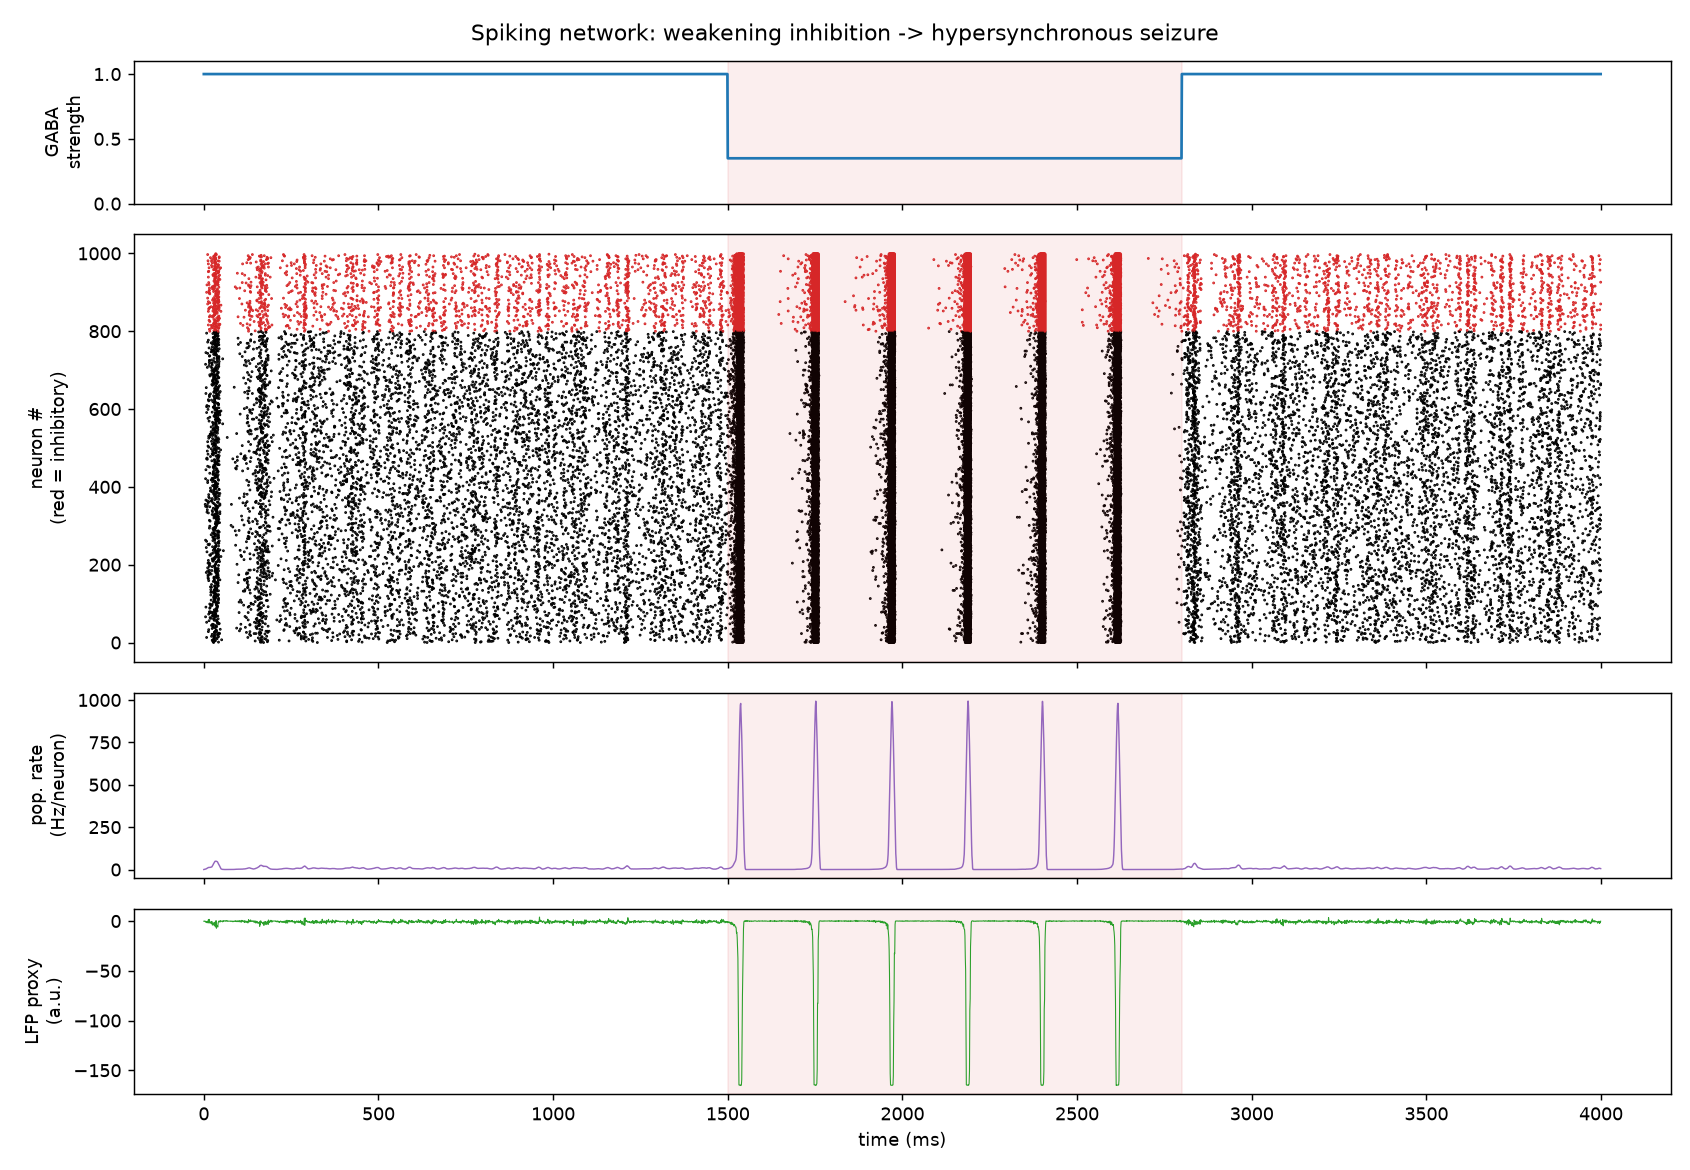
\includegraphics[width=0.75\linewidth]{epilepsy_sim/output/network_seizure.png}
\caption{Model 1: weakening inhibition turns asynchronous firing into lock-step population bursts.}
\label{fig:net}
\end{figure}

\begin{figure}[htbp]
\centering
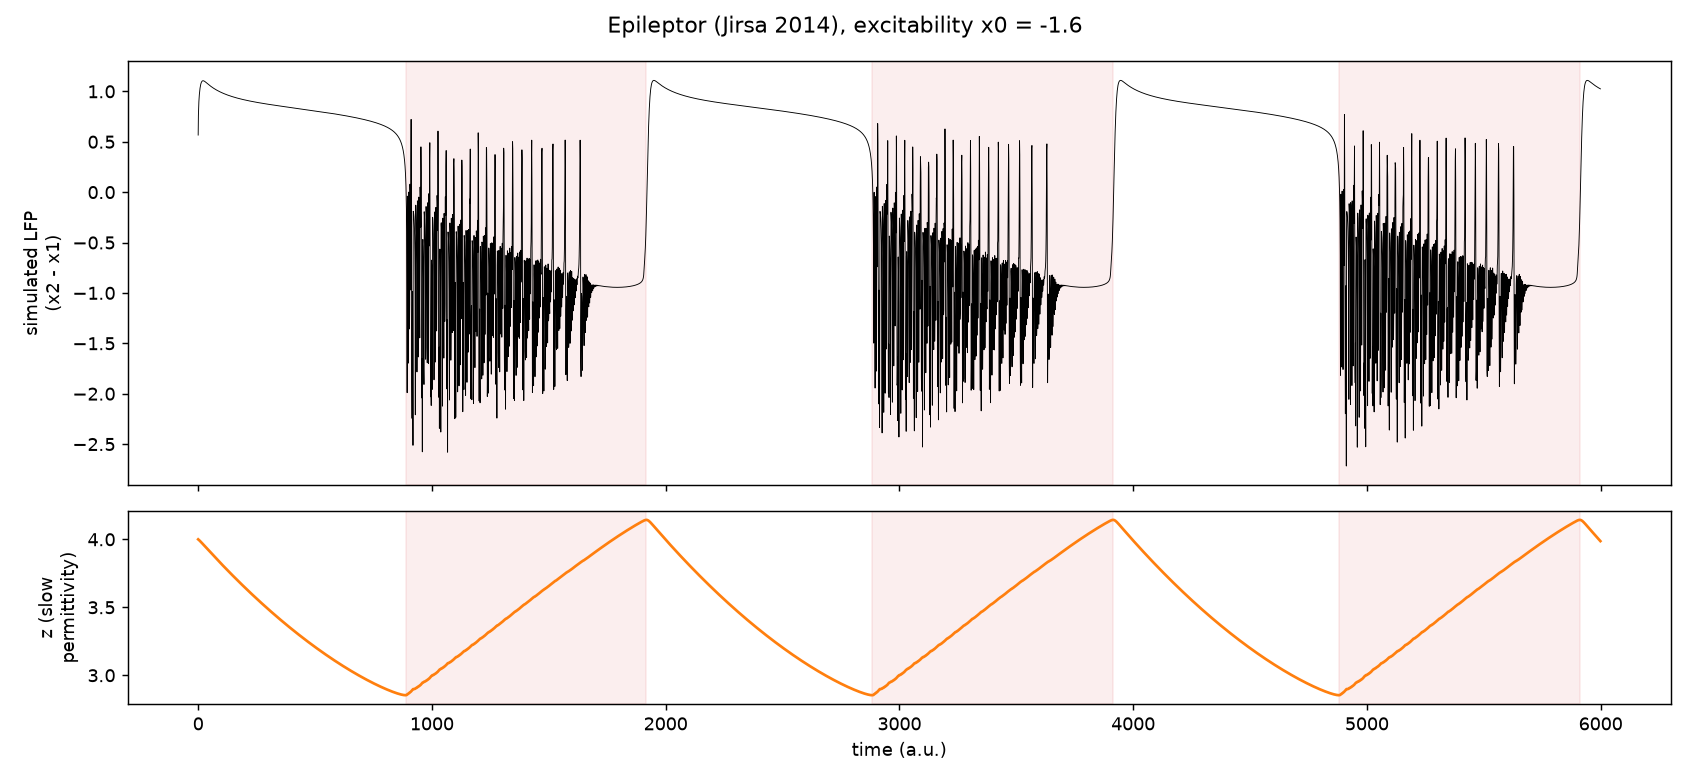
\includegraphics[width=0.75\linewidth]{epilepsy_sim/output/epileptor_seizures.png}
\caption{Model 2: Epileptor seizures driven by the slow permittivity variable $z$.}
\label{fig:epileptor}
\end{figure}

\paragraph{Model 3: validation.} In the reduced single-neuron configuration, the ionic model reproduced the periodic seizure-like events of \cite{cressman2009} (Table~\ref{tab:valid}, Figure~\ref{fig:valid}).

\begin{table}[htbp]
\centering\small
\caption{Validation against Cressman et al.\ (2009), Fig.~1.}
\label{tab:valid}
\begin{tabular}{@{}lll@{}}
\toprule
Quantity & Cressman 2009 & This implementation \\
\midrule
Seizure-like events & Periodic, every $\approx$30 s & Every $\approx$29.5 s \\
\Ko{} range & $\approx$6.7$\to$10.2 mM & 6.7$\to$10.7 mM \\
\Nai{} range & $\approx$16.3$\to$19 mM & 15.5$\to$19.1 mM \\
\bottomrule
\end{tabular}
\end{table}

\begin{figure}[htbp]
\centering
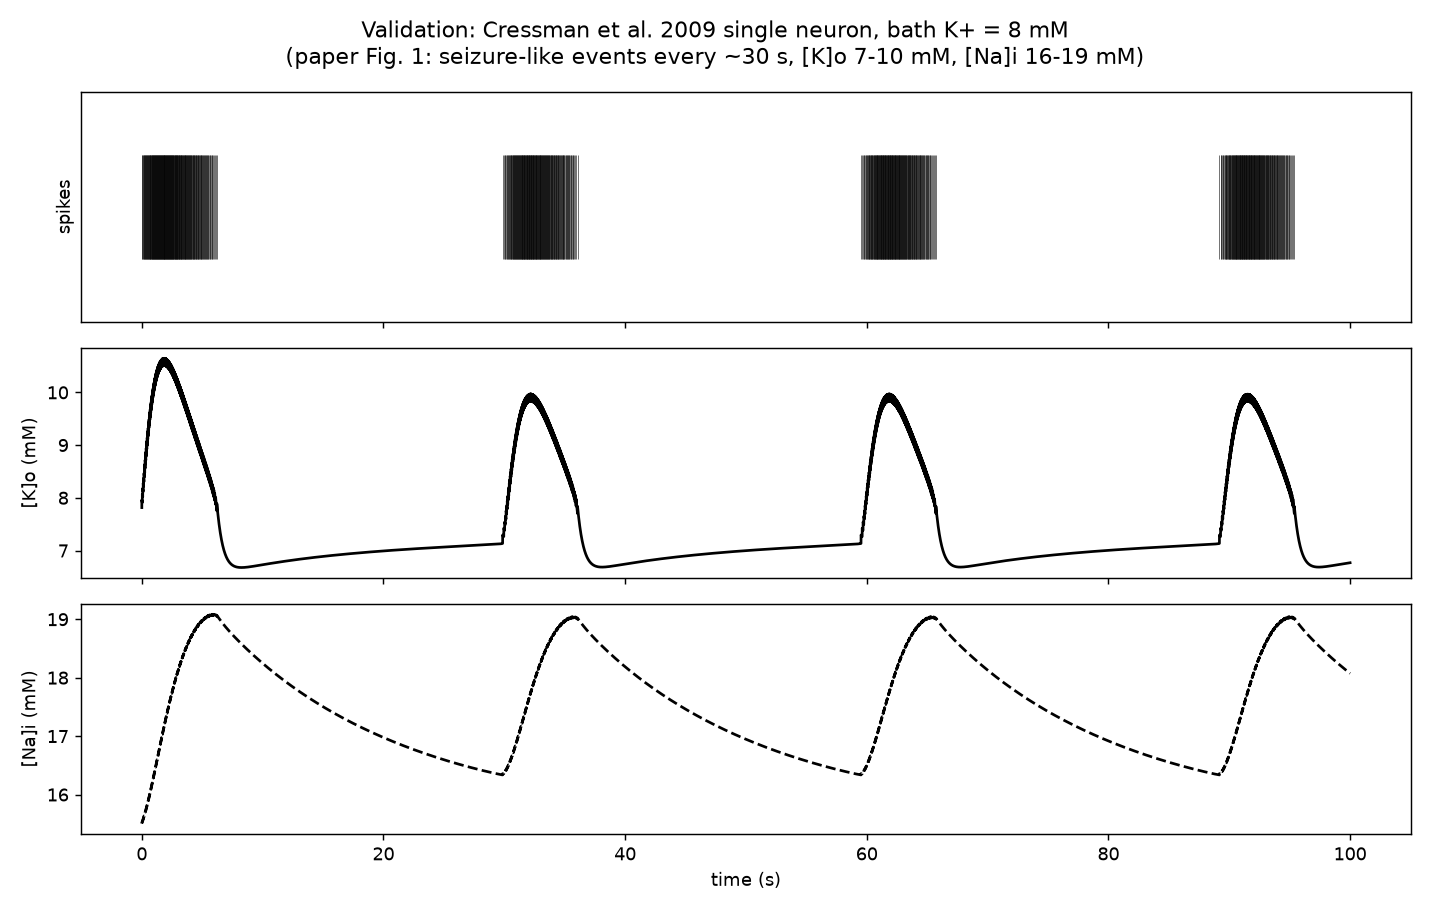
\includegraphics[width=0.65\linewidth]{epilepsy_sim/output/ionic_validation.png}
\caption{Single-neuron validation against Cressman et al.\ (2009), Fig.~1.}
\label{fig:valid}
\end{figure}

\paragraph{Model 3: healthy vs epileptic tissue.} With identical neurons, wiring and trigger, the pathological tissue showed every hallmark listed in Table~\ref{tab:ionic}; Figure~\ref{fig:ionic} shows the time courses.
\begin{itemize}
\item \textbf{Interictal state:} synchronous population bursts at $\approx$33/min, each sending local \Ko{} to 7--9\,mM with a saw-tooth in \Cli.
\item \textbf{Ictal event:} the trigger drove \Ko{} to the 12\,mM ceiling and \Cli{} to 15.2\,mM (\EGABA{} $-48.3$\,mV, so inhibition collapsed). Pump flux reached $\approx$1\,mM/s and adenosine 0.68, 5.7$\times$ the healthy peak.
\item \textbf{Postictal state:} a 25\,s silence, a \Kp{} undershoot to 3.66\,mM (as predicted by \cite{krishnan2011}) and a CBF fall to $-46$\%.
\end{itemize}
Healthy tissue capped \Ko{} near 6\,mM and recovered after a 13.7\,s pump after-hyperpolarisation. The ictal CBF peak was smaller in epileptic tissue because its baseline was already hyperactive.

\begin{table}[htbp]
\centering\small
\caption{Ionic model, healthy vs epileptic tissue (same neurons, wiring and trigger). \EGABA{} in the chord form.}
\label{tab:ionic}
\begin{tabularx}{\linewidth}{@{}l l l L@{}}
\toprule
Measure & Healthy & Epileptic & Physiological reference \\
\midrule
Baseline E firing & 6.1 Hz & 17.3 Hz & Hyperexcitable cortex \\
Resting \Cli{} & 5.6 mM & \best{11.6 mM} & Elevated in human epileptic tissue \\
Resting \EGABA{} & $-69.6$ mV & \best{$-54.1$ mV} & Depolarised with KCC2 loss \\
Resting \Ko{} & 4.18 mM & 4.59 mM & Impaired buffering \\
Interictal discharges & not epileptiform & \best{33/min} & IEDs on EEG \\
Peak \Ko{} (trigger) & 6.1 mM & \best{12.2 mM} & Ictal \Kp{} ceiling $\approx$10--12 mM \\
Peak \Cli{} & 7.4 mM & \best{15.2 mM} & Ictal \Clm{} loading \\
Peak \EGABA{} & $-63.7$ mV & \best{$-48.3$ mV} & Depolarising GABA \\
Peak \Nai{} & 26.2 mM & 29.8 mM & Ictal \Nap{} loading \\
Peak adenosine & 0.12 & \best{0.68} & Ictal adenosine surge \\
Postictal silence & 13.7 s & \best{25 s} & Postictal depression \\
Minimum \Ko{} after & 3.88 mM & \best{3.66 mM} & Postictal \Kp{} undershoot \\
CBF peak $\to$ minimum & +42\% $\to$ $-47$\% & +31\% $\to$ $-46$\% & Hyperperfusion then hypoperfusion \\
\bottomrule
\end{tabularx}
\end{table}

\begin{figure}[htbp]
\centering
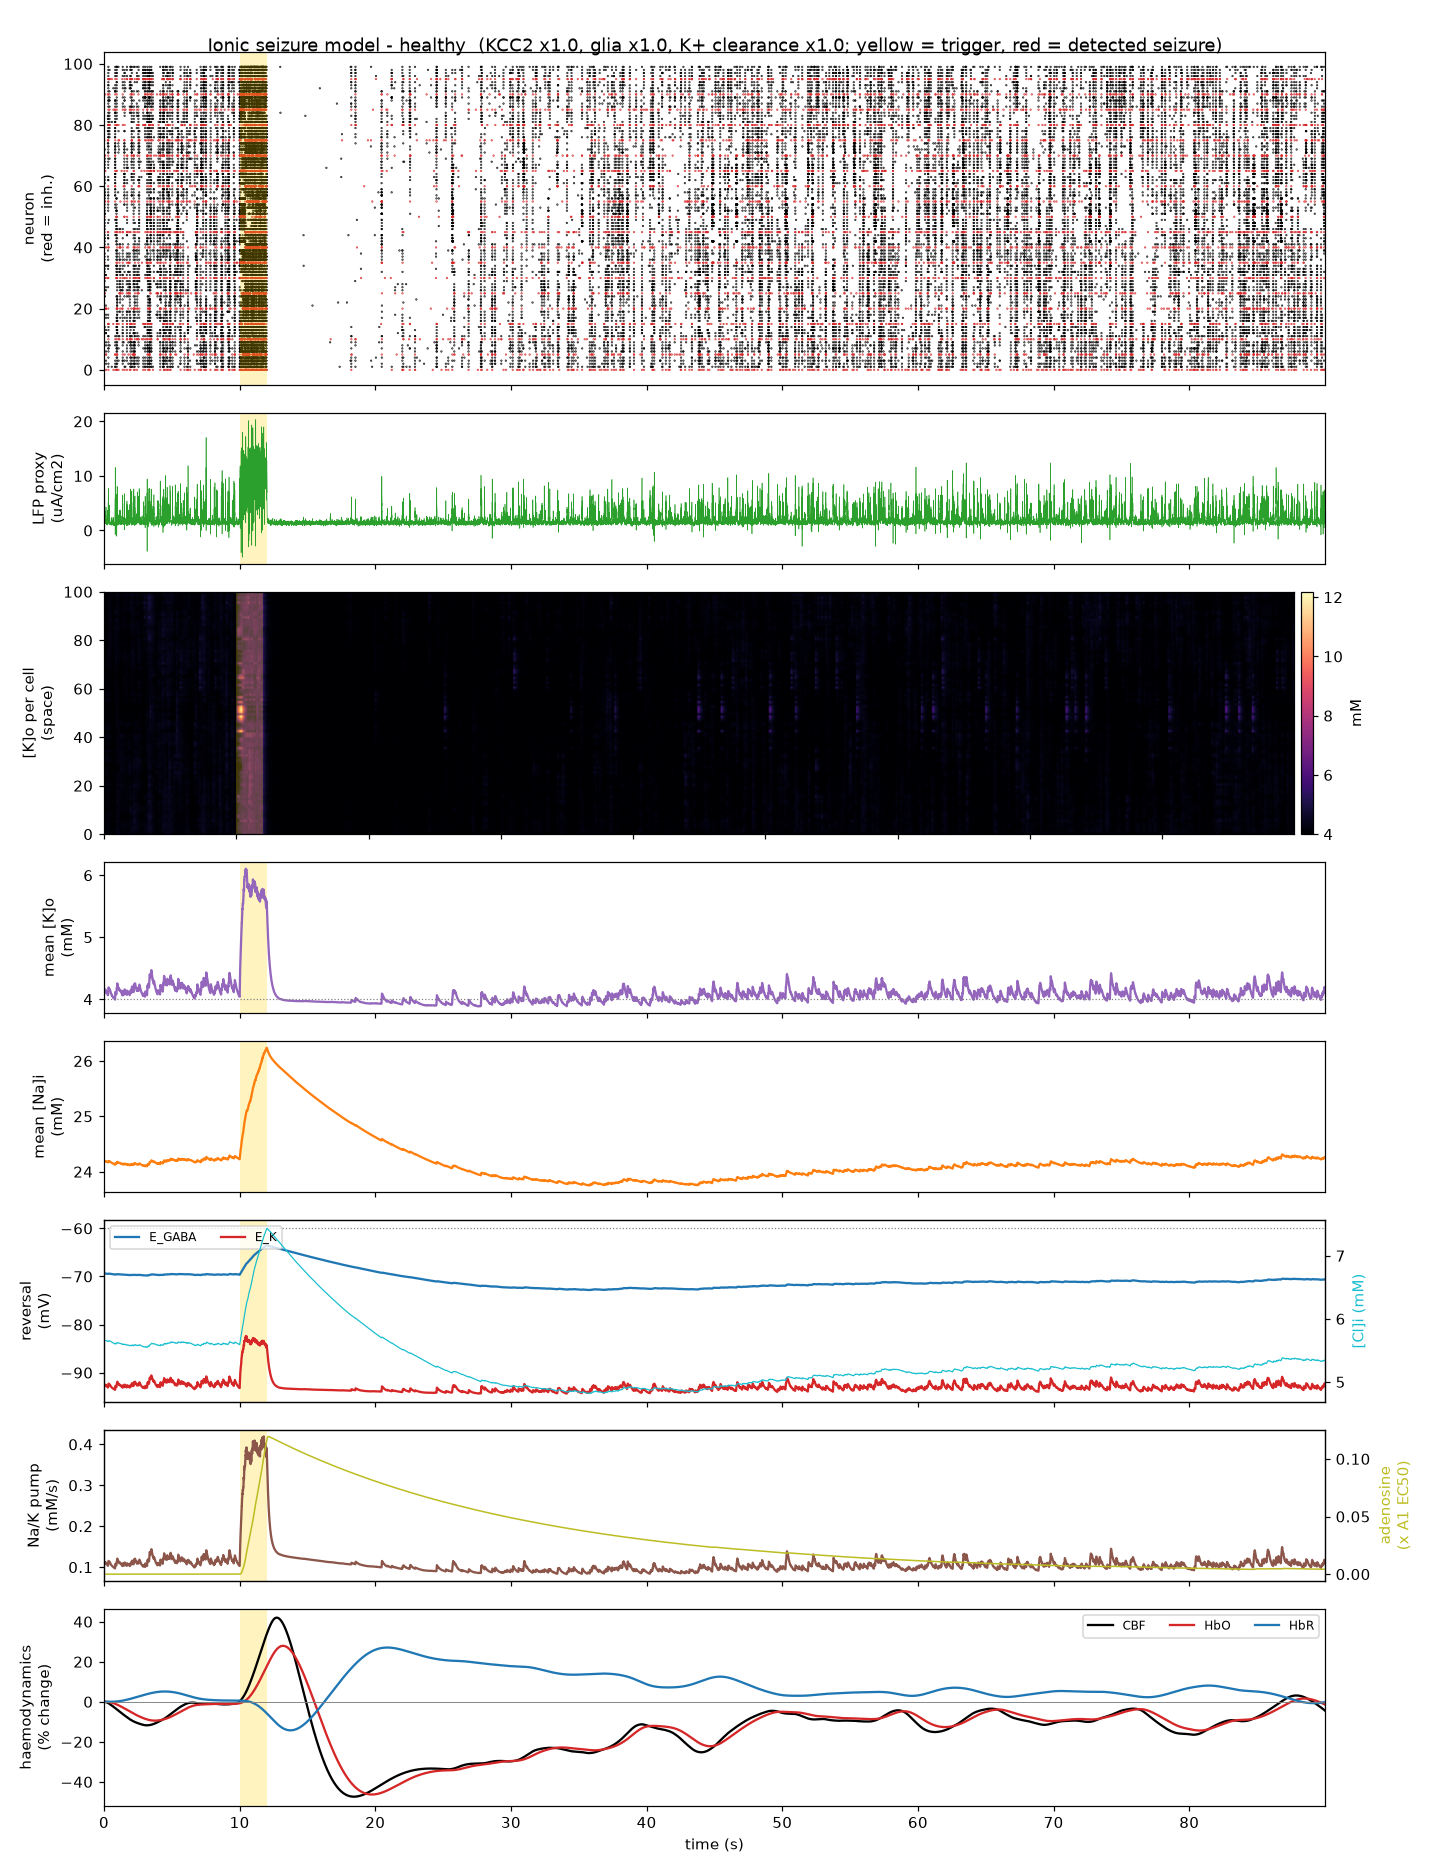
\includegraphics[width=0.49\linewidth]{epilepsy_sim/output/ionic_healthy.png}
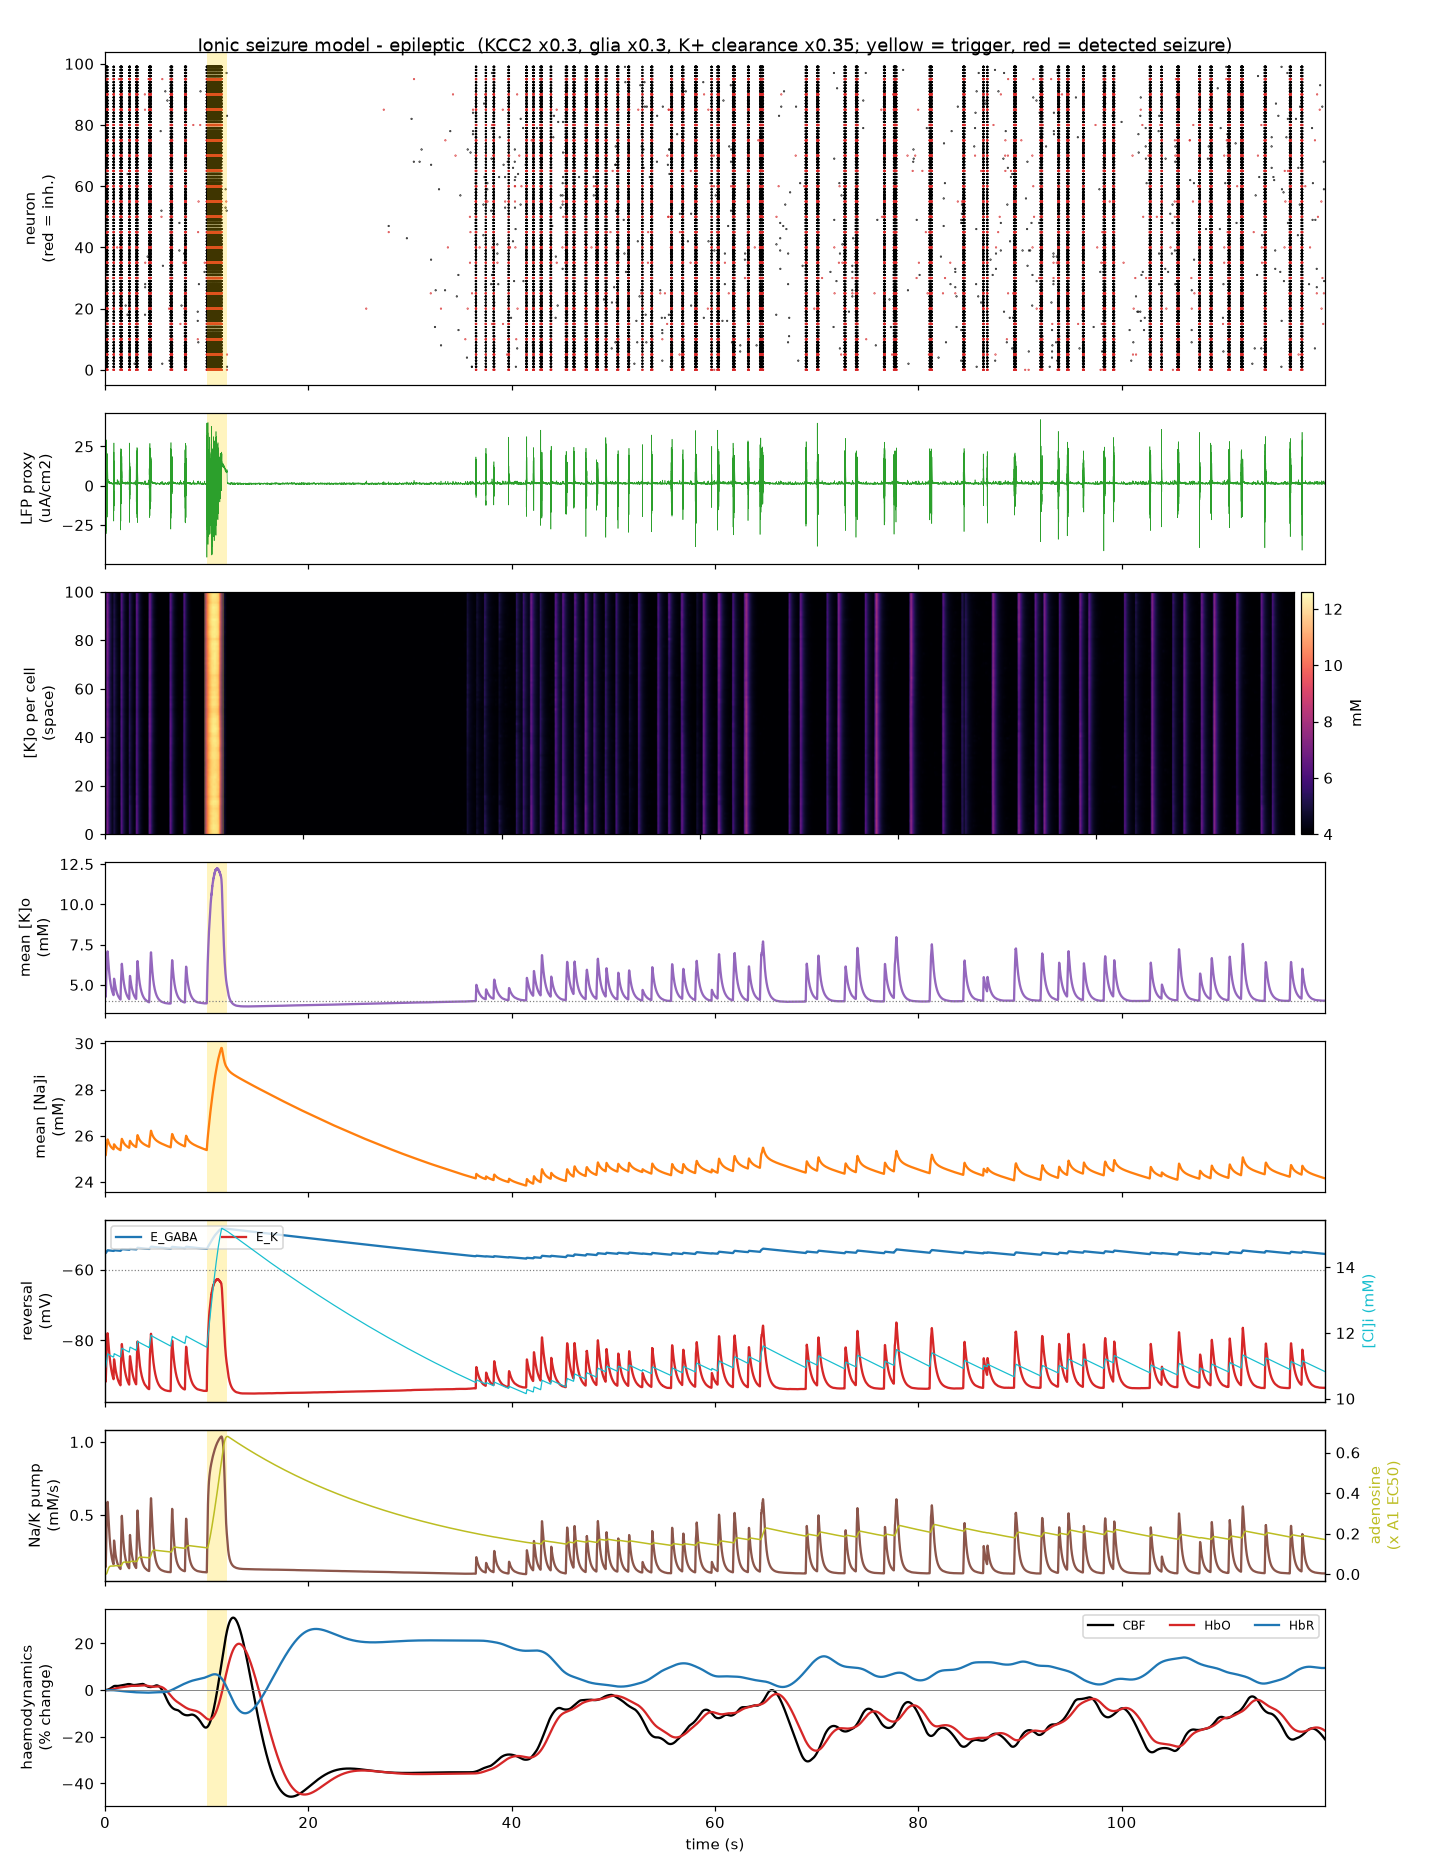
\includegraphics[width=0.49\linewidth]{epilepsy_sim/output/ionic_epileptic.png}
\caption{Ionic model, healthy (left) and epileptic (right) tissue. Panels show the raster, LFP proxy, space--time \Ko{} map, mean \Ko, \Nai, \EGABA/$E_K$/\Cli, pump flux and adenosine, and CBF/HbO/HbR.}
\label{fig:ionic}
\end{figure}

The model also reproduced KCC2-mediated \Kp{} loading and spatial spread by lateral diffusion. Its haemodynamic panel is what an optical sensor would record: a CBF/HbO surge, delayed by seconds, during the event, then a dip below baseline. Brief interictal events were nearly invisible optically. At the default pump setting, however, ictal events did not self-sustain beyond the trigger. Scaling the pump current down to 0.15 produced self-sustaining, self-terminating and recurring 10--20\,s seizures, but also made healthy tissue bistable (Appendix Table~\ref{tab:calib}).

% ----------------------------------------------------------------------------
\subsection{Inference of hidden variables}

\paragraph{E1: \Ko{} from a glial electrode.} With the textbook slope (61.54\,mV/decade), the RMSE was 0.239\,mM and the estimated peak 10.29\,mM (true 12.21, $-16$\%). With the measured slope (51), the RMSE fell to \textbf{0.062}\,mM and the peak was 12.32\,mM (+1\%).

\paragraph{E2: \Ko{} from DC-EEG.} The process model was calibrated on healthy data ($a=0.093$, $\tau=0.51$\,s) and applied to epileptic data with 3$\times$ slower clearance.
\begin{itemize}
\item Naive constant-gain conversion: RMSE 1.41\,mM, peak \textbf{29.2}\,mM (2.4$\times$ too high).
\item Activity-driven process model alone: RMSE 0.51\,mM (peak 14.1).
\item EKF combining process model and DC: RMSE \textbf{0.50}\,mM (peak 14.0), with estimated skull gain 0.015 (true 0.010).
\end{itemize}
With unknown gain and drift, the DC channel added little beyond the EEG-driven model.

\paragraph{E3: \Cli{} from \EGABA.} The chord inverse gave RMSE \textbf{1.12}\,mM (bias $-0.13$). The GHK inverse was biased:
\begin{itemize}
\item $r=0.20$: RMSE 3.05, bias \textbf{+2.72};
\item $r=0.25$: RMSE 2.50, bias +2.09;
\item $r=0.44$: RMSE 1.47, bias $-0.32$ (a coincidental crossing).
\end{itemize}
With the correct formula, $\pm$2\,mV of \EGABA{} error became $\approx\pm$1.1\,mM of chloride error. That is enough to separate healthy (5.6\,mM) from epileptic (11.6\,mM) tissue.

\paragraph{E4: E/I from the spectrum.} The 30--50\,Hz fit gave $\chi=1.65$ in healthy tissue ($R^2$ 0.87) vs 1.50 in epileptic tissue (0.75), the direction associated with more excitation. The broadband 2--200\,Hz knee fit failed in epileptic tissue ($\chi\approx0$, $R^2$ 0.74) because interictal spikes inject high-frequency power.

\paragraph{E5: HbO/HbR from fNIRS.}
\begin{itemize}
\item Naive MBLL: RMSE 10.3\,\uM, $r=0.873$, recovered amplitude 22\%.
\item With short-channel regression: $r=$ \textbf{0.996}, amplitude 16\%.
\item With partial-volume correction added: RMSE \textbf{1.40}\,\uM, amplitude 1.10; the residual +10\% equals the injected DPF error.
\item HbR, full pipeline: RMSE 0.49\,\uM, $r=0.999$.
\end{itemize}
A temple PPG device without a short channel and depth resolution would underestimate cortical changes about 5$\times$.

\paragraph{E6: adenosine.} The decay law $A_{peak}e^{-T/20}$ reproduced adenosine at recovery exactly (0.060 vs 0.061 healthy; 0.195 vs 0.196 epileptic). However, the level at which firing resumed differed 3.2$\times$ between tissues, so no universal threshold exists and the closed-form formula was withdrawn.

\paragraph{E7: KCC2 strength.} Table~\ref{tab:e7} shows the posterior. Its mean was \textbf{0.36$\pm$0.09} (true 0.30). The MAP fell on 0.45 because the noisy \EGABA{} ``measurement'' was $-55.3$ vs $-54.0$\,mV. \EGABA{} carried almost all of the information, since rate was non-monotonic in KCC2. Healthy and severe-loss values were correctly ruled out; 0.3 vs 0.45 could not be separated.

\begin{table}[htbp]
\centering\small
\caption{E7: posterior over KCC2 strength (true 0.3).}
\label{tab:e7}
\begin{tabular}{@{}lcccccc@{}}
\toprule
KCC2 ($\times$ normal) & 0.15 & 0.2 & \textbf{0.3} & 0.45 & 0.7 & 1.0 \\
\midrule
Simulated \EGABA{} (mV) & $-51.3$ & $-52.5$ & $-54.2$ & $-56.4$ & $-60.7$ & $-63.5$ \\
Simulated E rate (Hz) & 13.2 & 12.4 & 9.9 & 12.2 & 10.3 & 10.9 \\
Posterior & 0.014 & 0.103 & \textbf{0.414} & \textbf{0.468} & 0.001 & $\approx$0 \\
\bottomrule
\end{tabular}
\end{table}

\begin{figure}[htbp]
\centering
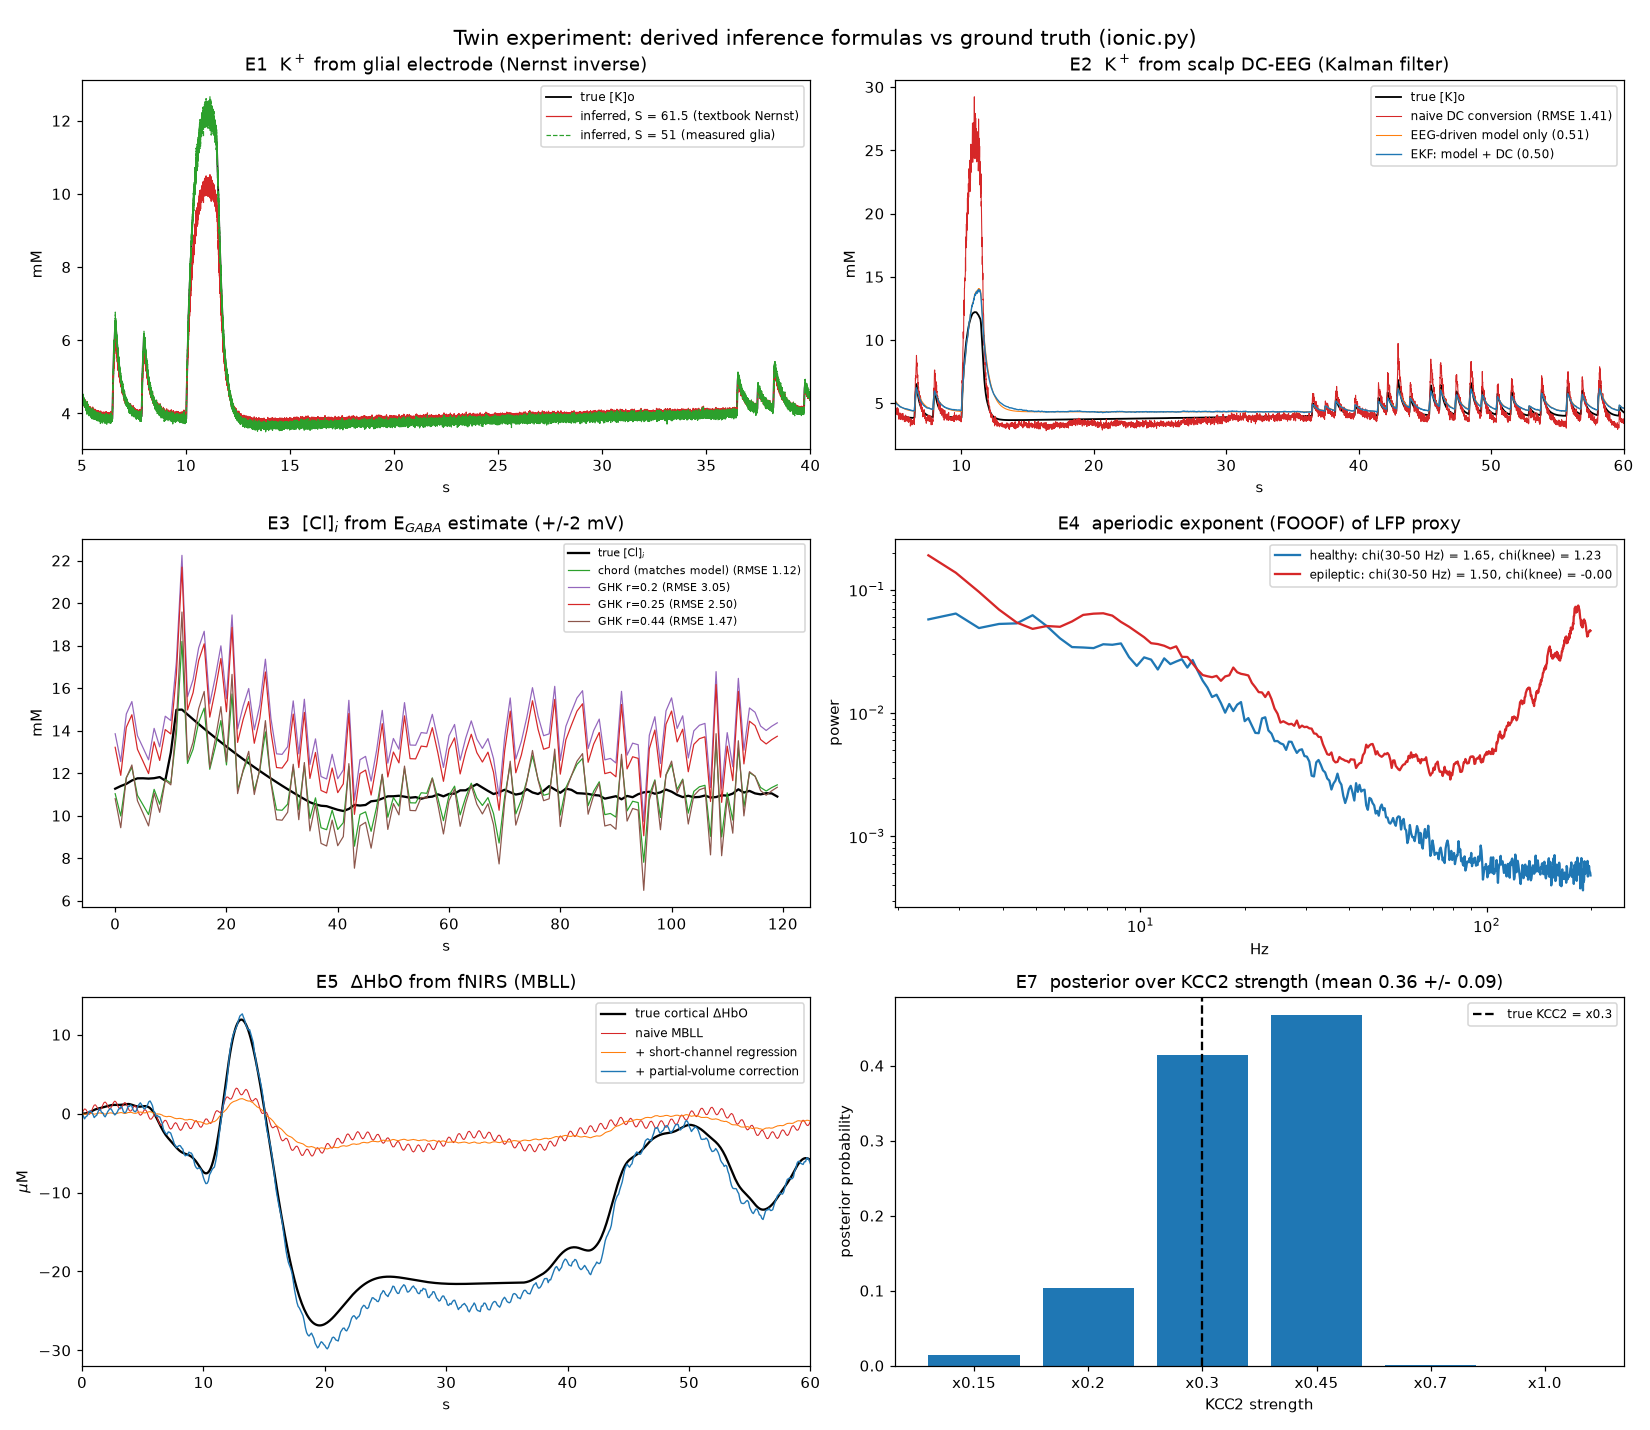
\includegraphics[width=0.82\linewidth]{epilepsy_sim/output/infer_results.png}
\caption{Twin experiments E1--E7.}
\label{fig:twin}
\end{figure}

\paragraph{T1: Epileptor vs TVB.} The first onset was identical (886.2), and all differences shrank with the time step (Table~\ref{tab:t1}). The residual discrepancy therefore comes from the integrator (Euler vs Heun), not from the model. Our implementation was 7--30$\times$ faster for a single region.

\begin{table}[htbp]
\centering\small
\caption{T1: cross-validation of our Epileptor against TVB.}
\label{tab:t1}
\begin{tabular}{@{}llll@{}}
\toprule
& TVB (Heun, dt 0.05) & Ours (Euler, dt 0.05) & Ours (Euler, dt 0.01) \\
\midrule
Seizures in 6000 a.u. & 3 & 3 & 3 \\
Onsets & 886.2, 2820.2, 4754.2 & 887.0, 2883.0, 4880.0 & \textbf{886.2}, 2827.6, 4769.0 \\
Seizure duration & 968.7 & 1030 & \textbf{976.2} \\
$z$ RMSE vs TVB & -- & 0.139 & \textbf{0.018} \\
LFP correlation & -- & 0.71 & 0.87 \\
Runtime & 43 s & 1.5 s & 6.4 s \\
\bottomrule
\end{tabular}
\end{table}

\paragraph{T2: whole-brain inference.} The epileptogenic zone seized first (onset 1022\,ms, recurring every $\approx$1.4\,s). The seizure spread to \textbf{36 of 38} right-hemisphere regions and to none on the left. From onset times alone, the zone was localised correctly and its excitability recovered as $-1.60\pm0.0002$ (posterior $8\times10^{-8}$ at $-1.7$ and $3\times10^{-6}$ at $-1.5$). This is an \emph{inverse crime}: the same model, parameters and grid generated and fitted the data, so the posterior collapsed unrealistically (Figure~\ref{fig:tvb}).

\begin{figure}[htbp]
\centering
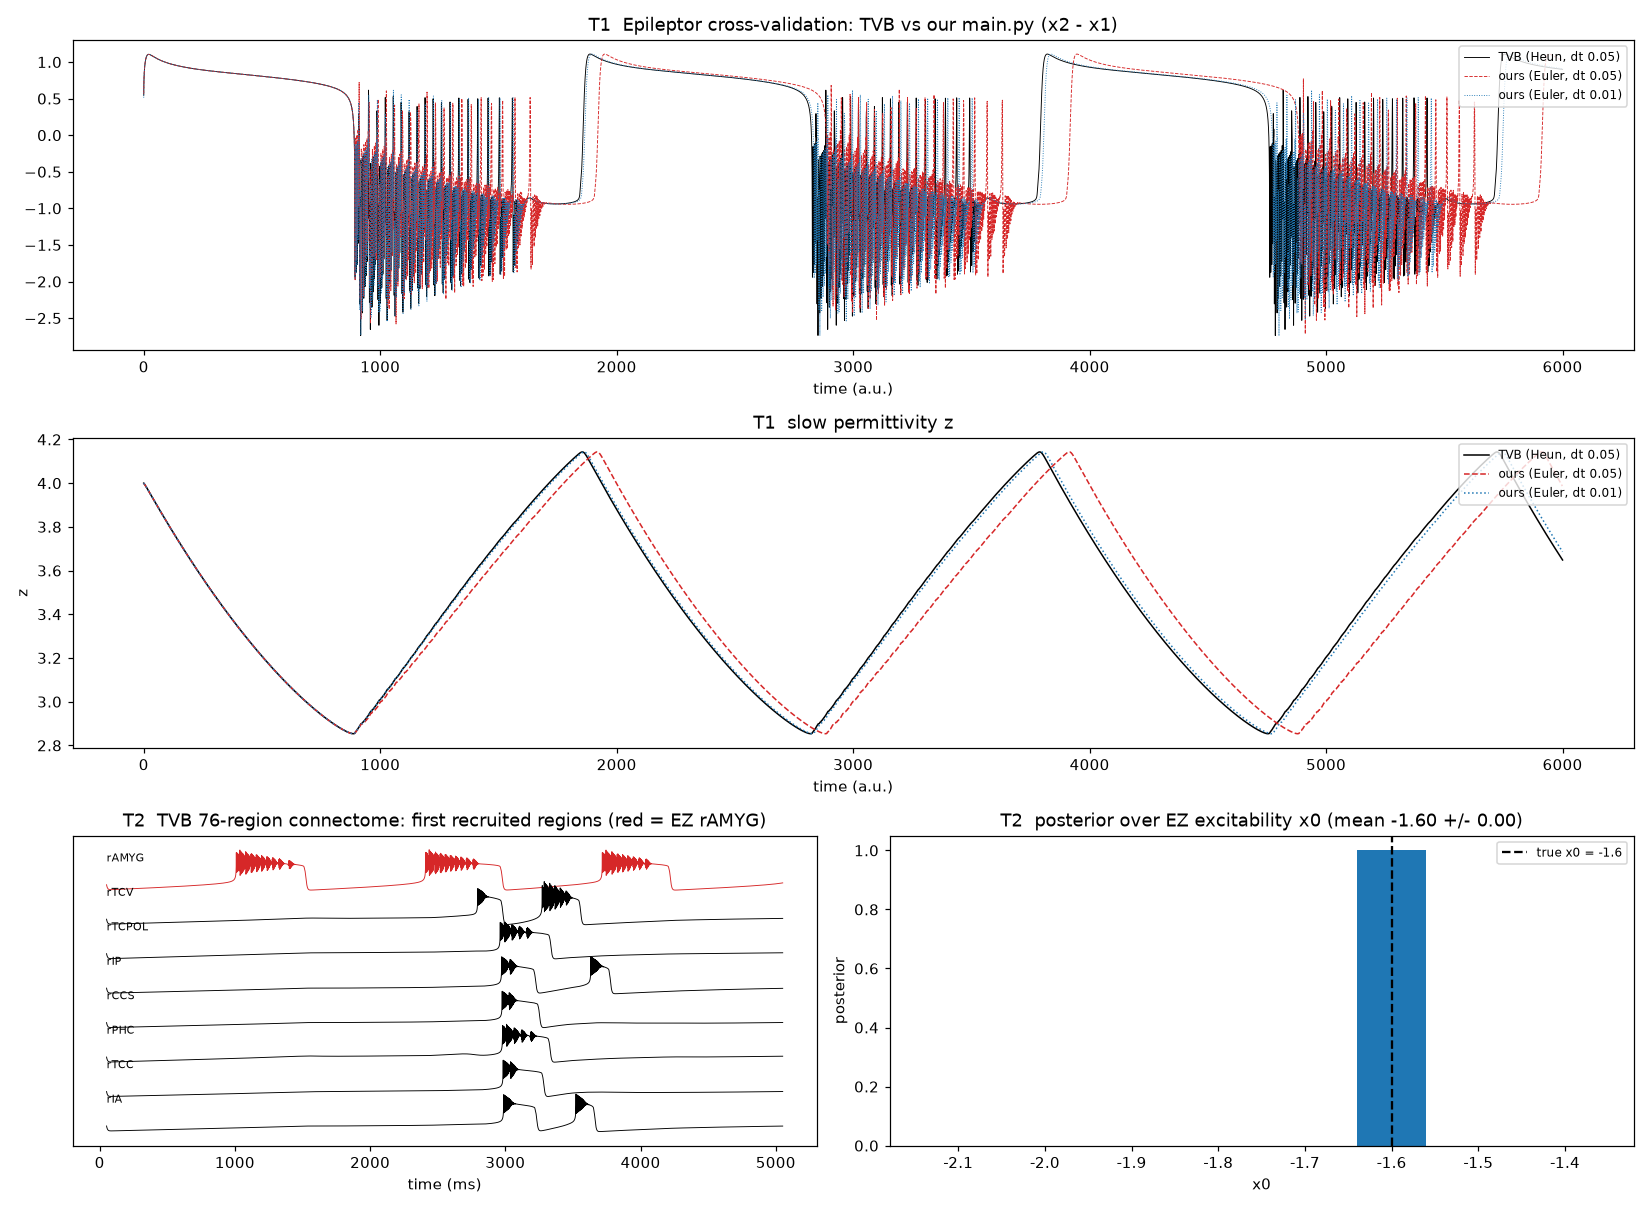
\includegraphics[width=0.82\linewidth]{epilepsy_sim/output/tvb_compare.png}
\caption{TVB cross-validation (T1) and VEP-style whole-brain inference (T2).}
\label{fig:tvb}
\end{figure}

% ----------------------------------------------------------------------------
\subsection{Scalp-EEG montage study (CHB-MIT)}

\paragraph{Patient-specific models.} Every temple montage caught all 19 seizures (Table~\ref{tab:chb3}, Figure~\ref{fig:chb3}). Both temples produced 9.8 \FAd{}, against 5.2 for the full cap. One-sided montages produced 3--6$\times$ more false alarms than bilateral ones. Cross-patient models trained on only two patients generalised poorly (205--414 \FAd). With 36.6\,h of data, one false alarm corresponds to 0.66/day, so these rates are coarse.

\begin{table}[htbp]
\centering\small
\caption{CHB-MIT, 3 patients (19 seizures, 36.6 h), threshold 0.5.}
\label{tab:chb3}
\begin{tabular}{@{}lcccccc@{}}
\toprule
& \multicolumn{3}{c}{Patient-specific} & \multicolumn{3}{c}{Cross-patient} \\
\cmidrule(lr){2-4}\cmidrule(lr){5-7}
Montage & Caught & FA/day & Latency & Caught & FA/day & Latency \\
\midrule
Full cap (18 ch) & 95\% (18/19) & \textbf{5.2} & 4.5 s & 37\% & 273.8 & 3.0 s \\
Both temples (4 ch) & \textbf{100\%} (19/19) & 9.8 & 6.0 s & 63\% & 306.6 & 18.0 s \\
Right temple (2 ch) & 100\% & 36.0 & 5.0 s & 84\% & 205.0 & 12.5 s \\
Left temple (2 ch) & 100\% & 32.1 & 10.0 s & 79\% & 414.0 & 17.0 s \\
Right temple (1 ch) & 100\% & 62.9 & 5.0 s & 100\% & 226.0 & 8.0 s \\
\bottomrule
\end{tabular}
\end{table}

\begin{figure}[htbp]
\centering
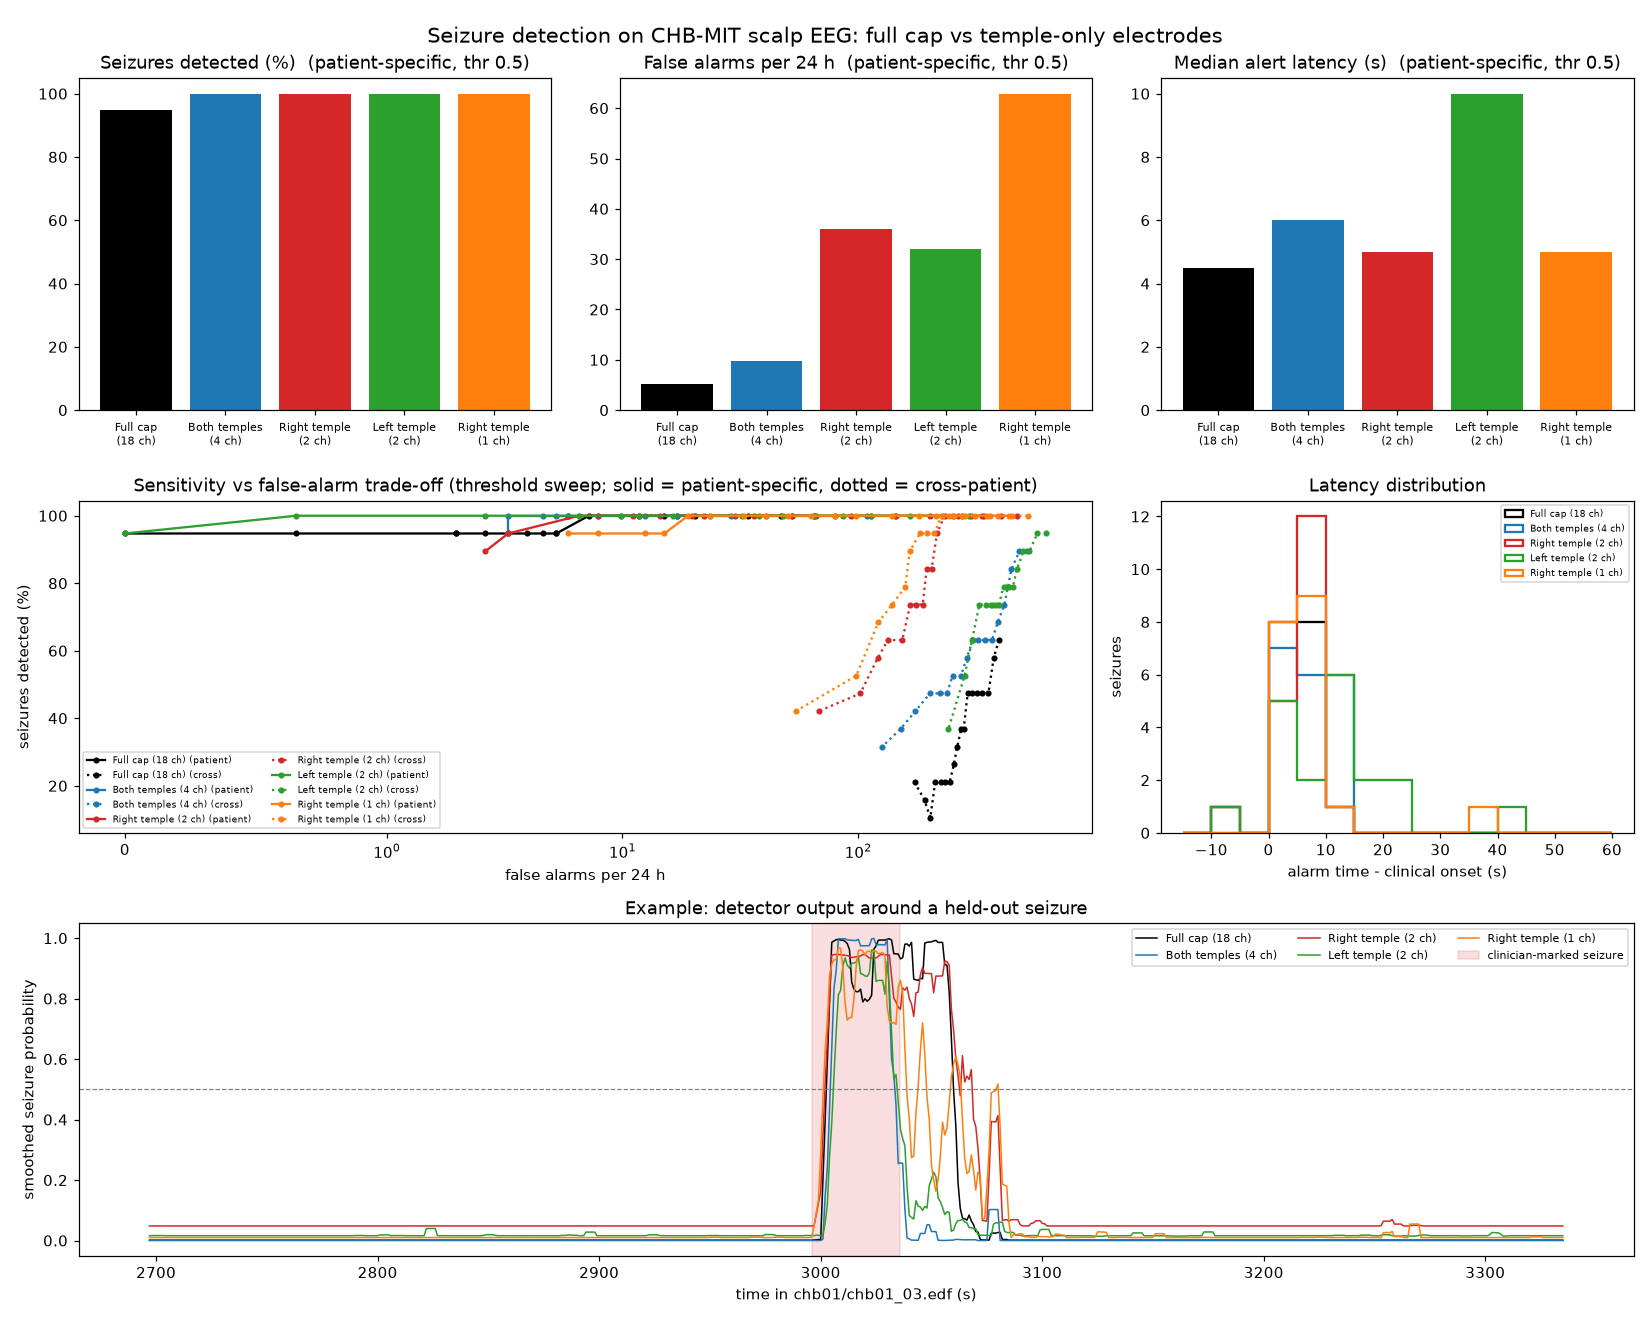
\includegraphics[width=0.78\linewidth]{epilepsy_sim/detect/results/detection.png}
\caption{CHB-MIT patient-specific detection by montage.}
\label{fig:chb3}
\end{figure}

\paragraph{General model for new users.} Per-person normalisation raised temple-montage sensitivity from 62\% to 85\% (43 more seizures) while reducing false alarms (Table~\ref{tab:general}). The two-channel ear-hook caught as many seizures as the 18-channel cap (88\% vs 85\%) with lower median latency. It produced $\approx$1.7$\times$ the false alarms (382 vs 229 \FAd). Using both ears instead of one added about 6\% more seizures and reduced false alarms by 25--30\%.

\begin{table}[htbp]
\centering\small
\caption{CHB-MIT general model, new users (leave-one-subject-out; 23 subjects, 185 seizures), threshold 0.5.}
\label{tab:general}
\begin{tabular}{@{}lccc@{}}
\toprule
Montage & Caught & FA/day & Median latency \\
\midrule
Temple (4 ch), raw features & 62\% (114/185) & 525 & 6.5 s \\
Temple (4 ch), per-person normalised & 85\% (157/185) & 342 & 6.0 s \\
\textbf{Ear-hook both ears (2 ch)}, normalised & \textbf{88\%} (162/185) & 382 & \textbf{5.0 s} \\
Ear-hook one ear (1 ch), normalised & 83\% (154/185) & 556 & 6.0 s \\
Full cap (18 ch), normalised & 85\% (157/185) & \textbf{229} & 5.0 s \\
\bottomrule
\end{tabular}
\end{table}

\paragraph{Fine-tuning.} Fine-tuning on two of the user's own seizure recordings cut false alarms by 40--65\% without losing seizures (Table~\ref{tab:generalft}, Figure~\ref{fig:general}). Patient-only models had few false alarms but missed about a third of seizures. At stricter thresholds, chosen post hoc and therefore optimistic, fine-tuned detectors reached $\approx$18--23 \FAd{} while catching 64\% (ear-hook, both ears) to 75\% (full cap) of seizures.

\begin{table}[htbp]
\centering\small
\caption{Fine-tuning on the first $k$ seizure recordings (caught / FA per day on later recordings).}
\label{tab:generalft}
\begin{tabular}{@{}llccc@{}}
\toprule
Montage & $k$ & General only & Patient-only & General + fine-tuned \\
\midrule
Temple (4 ch) & 1 & 84\% / 351 & 53\% / 8 & 83\% / 162 \\
 & 2 & 84\% / 361 & 68\% / 16 & \textbf{86\% / 138} \\
Ear-hook both ears (2 ch) & 1 & 86\% / 385 & 54\% / 9 & 83\% / 186 \\
 & 2 & 87\% / 397 & 65\% / 18 & \textbf{86\% / 162} \\
Ear-hook one ear (1 ch) & 1 & 81\% / 547 & 44\% / 13 & 74\% / 241 \\
 & 2 & 81\% / 550 & 66\% / 79 & 80\% / 216 \\
Full cap (18 ch) & 1 & 83\% / 240 & 56\% / 3 & 84\% / 95 \\
 & 2 & 84\% / 246 & 68\% / 6 & \textbf{89\% / 88} \\
\bottomrule
\end{tabular}
\end{table}

\begin{figure}[htbp]
\centering
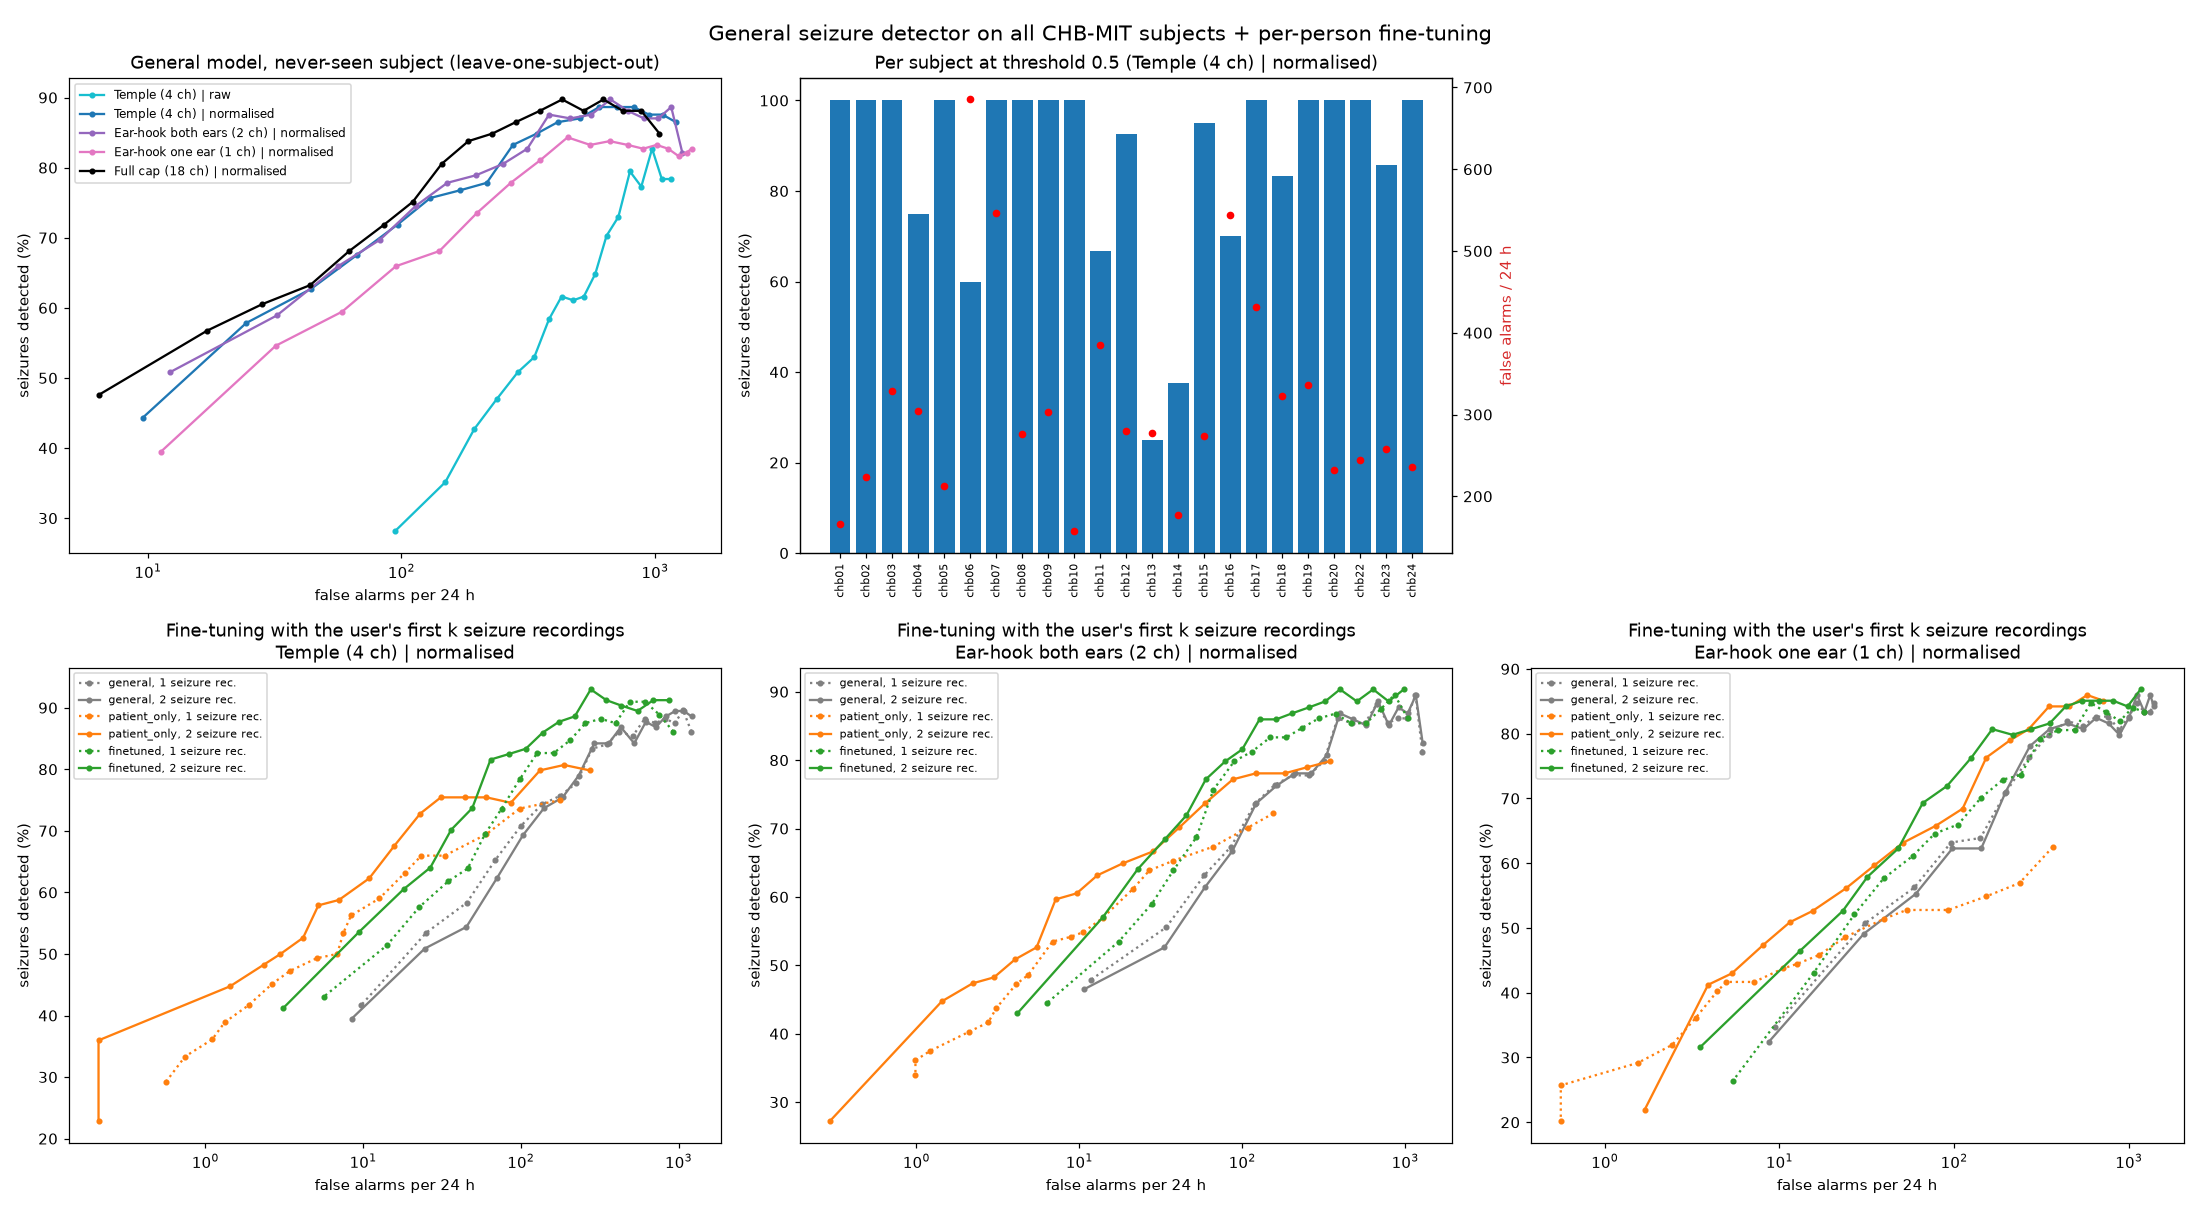
\includegraphics[width=0.95\linewidth]{epilepsy_sim/detect/results_general/general.png}
\caption{CHB-MIT general model on all subjects and personal fine-tuning.}
\label{fig:general}
\end{figure}

% ----------------------------------------------------------------------------
\subsection{Multimodal wearable study (SeizeIT2)}

\paragraph{Modalities.} Adding ECG to ear EEG reduced false alarms by 18\%, 24\% and 31\% at 50\%, 60\% and 70\% sensitivity (Table~\ref{tab:sz2main}). It also raised the share of seizures caught at $\le$5 \FAd{} from 14\% to 21\% (Table~\ref{tab:sz2budget}).

Per patient, the median false-alarm rate at threshold 0.5 fell with each added modality:
\begin{itemize}
\item EEG only: 618 (IQR 533--686);
\item EEG+ECG: 373 (329--440);
\item all four modalities: 342 (299--400).
\end{itemize}
EEG+ECG had fewer false alarms than EEG alone in \textbf{115/125} patients (all four: 120/125), while detections per patient barely changed (more in 16 patients, fewer in 21). ECG alone rivalled ear EEG under strict budgets. EMG and motion, used as direct features, gave no consistent gain for these mostly non-convulsive seizures. Two interim snapshots taken during streaming (48 patients: $-7$\% to $-20$\%; 78 patients: $-21$\% to $-44$\%) converged to the final estimate.

\begin{table}[htbp]
\centering\small
\caption{SeizeIT2 (125 patients, 883 seizures): false alarms per 24 h at matched sensitivity (lower is better). Percentages are relative to EEG only.}
\label{tab:sz2main}
\begin{tabular}{@{}lcccc@{}}
\toprule
Setup & 50\% caught & 60\% & 70\% & 80\% \\
\midrule
EEG only (ear) & 103.7 & 161.7 & 294.4 & not reached \\
ECG only & 132.6 & 225.6 & 378.2 & 677.8 \\
Body only (ECG+EMG+motion) & 116.3 & 193.5 & 283.8 & 583.1 \\
\textbf{EEG + ECG} & \textbf{85.5} ($-18$\%) & \textbf{122.8} ($-24$\%) & \textbf{204.0} ($-31$\%) & \textbf{459.2} \\
EEG + ECG + EMG + motion & 75.4 ($-27$\%) & 139.3 ($-14$\%) & 211.7 ($-28$\%) & 539.9 \\
\bottomrule
\end{tabular}
\end{table}

\begin{table}[htbp]
\centering\small
\caption{Seizures caught within a daily false-alarm budget, and at the default threshold 0.5.}
\label{tab:sz2budget}
\setlength{\tabcolsep}{4.5pt}
\begin{tabular}{@{}lccccc|ccc@{}}
\toprule
Setup & $\le$5 & $\le$20 & $\le$50 & $\le$100 & $\le$200 & Caught @0.5 & FA/day & Latency \\
\midrule
EEG only & 14\% & 23\% & 23\% & 42\% & 62\% & 79.4\% & 608 & 6 s \\
ECG only & 16\% & 29\% & 29\% & 48\% & 60\% & 74.0\% & 438 & 7 s \\
Body only & 16\% & 28\% & 42\% & 50\% & 64\% & 75.4\% & 386 & 8 s \\
\textbf{EEG + ECG} & \textbf{21\%} & \textbf{35\%} & 35\% & \textbf{57\%} & 66\% & 78.7\% & \textbf{399} & 7 s \\
All four & 20\% & 34\% & \textbf{45\%} & 53\% & \textbf{68\%} & 78.3\% & 348 & 7 s \\
\bottomrule
\end{tabular}
\end{table}

\paragraph{Context and HR-excess.} Minute-scale context and HR-excess each reduced false alarms, and combined they gave the best general model (Table~\ref{tab:ctx}, Figure~\ref{fig:sz2}). Relative to ear EEG alone, it had $-62$\%, $-43$\% and $-47$\% false alarms at 50\%, 60\% and 70\% sensitivity, and it caught 28\% of seizures at $\le$5 \FAd.

HR-excess alone reduced false alarms by 42\% at 50\% sensitivity. This was despite a univariate pre-check that suggested little value (AUC 0.62 vs 0.61 for raw HR in separating false alarms from detections).

The bigger model gave mixed results at 3$\times$ the compute, which indicates that model capacity and training-set size were not the bottleneck.

\begin{table}[htbp]
\centering\small
\caption{Context and HR-excess configurations (125 patients, general model): FA/day at matched sensitivity and seizures caught within budgets.}
\label{tab:ctx}
\setlength{\tabcolsep}{4.5pt}
\begin{tabular}{@{}lccccccc@{}}
\toprule
Setup & 50\% & 60\% & 70\% & 80\% & $\le$5/d & $\le$50/d & $\le$200/d \\
\midrule
Ear EEG only & 103.7 & 161.7 & 294.4 & -- & 14\% & 23\% & 62\% \\
EEG + context & 72.2 & 148.2 & 287.7 & 770.6 & 21\% & 48\% & 65\% \\
EEG + ECG & 85.5 & 122.8 & 204.0 & 459.2 & 21\% & 35\% & 66\% \\
EEG + ECG + context & 59.5 & 98.5 & 194.6 & 401.8 & 25\% & 48\% & 72\% \\
EEG + ECG + HR-excess & 49.2 & 111.7 & 177.7 & 385.8 & 20\% & 50\% & 72\% \\
\textbf{EEG + ECG + context + HR-excess} & \textbf{39.6} & \textbf{92.5} & \textbf{154.9} & \textbf{368.0} & \textbf{28\%} & \textbf{50\%} & \textbf{73\%} \\
same, big model & 48.2 & 82.8 & 165.0 & 500.6 & 25\% & 54\% & 72\% \\
EEG + PPG(sim) + context + HR-excess & 44.8 & 83.5 & 175.2 & 376.5 & 26\% & 53\% & -- \\
\bottomrule
\end{tabular}
\end{table}

\begin{figure}[htbp]
\centering
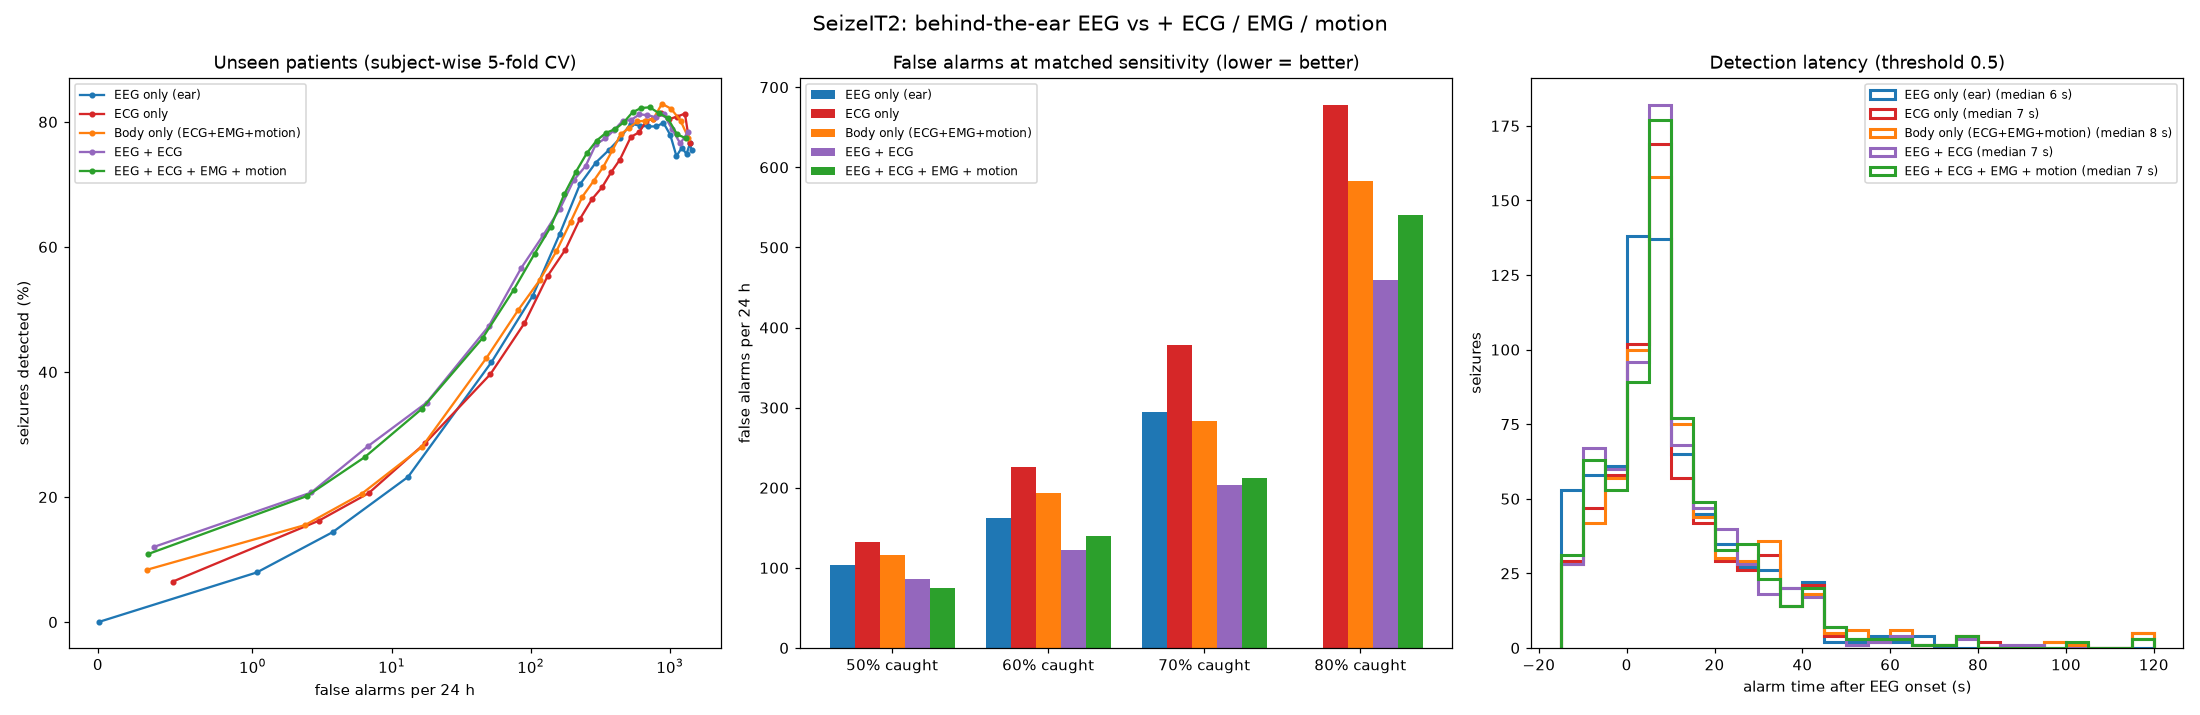
\includegraphics[width=\linewidth]{epilepsy_sim/detect/results_seizeit2/seizeit2.png}
\caption{SeizeIT2: sensitivity vs false alarms, false alarms at matched sensitivity, and latency for all configurations.}
\label{fig:sz2}
\end{figure}

\paragraph{Personal fine-tuning.} With two tuning seizures (71 patients), ECG and fine-tuning reduced false alarms at 50\% sensitivity by 44\% and 42\% respectively. Together they reduced them by 62\%, close to the 67\% expected for independent effects, with no change in delay (Table~\ref{tab:ft}). With a single tuning seizure, EEG-only tuning was inconsistent: better at 40\% sensitivity, worse at 60\% and under strict budgets. With ECG, even one seizure helped ($-16$\% to $-45$\%). Requiring 10 or 20\,s sustained above threshold helped only at low sensitivity, was worse at 60--70\%, and added 3--7\,s of delay.

\begin{table}[htbp]
\centering\small
\caption{Fine-tuning on 2 own seizures (71 patients, later data): FA/day at matched sensitivity and seizures caught within budgets.}
\label{tab:ft}
\begin{tabular}{@{}lccccccc@{}}
\toprule
Setup & 40\% & 50\% & 60\% & 70\% & $\le$1/d & $\le$5/d & $\le$20/d \\
\midrule
EEG, general & 100.8 & 157.9 & 221.3 & 289.0 & 0\% & 11\% & 20\% \\
EEG, fine-tuned & 61.5 & 91.6 & 127.9 & 217.1 & 8\% & 15\% & 28\% \\
EEG+ECG, general & 52.4 & 88.7 & 168.0 & 254.7 & 10\% & 18\% & 32\% \\
\textbf{EEG+ECG, fine-tuned} & \textbf{40.5} & \textbf{60.5} & \textbf{107.2} & \textbf{192.5} & \textbf{14\%} & \textbf{21\%} & 27\% \\
\bottomrule
\end{tabular}
\end{table}

\paragraph{Personal thresholds and calibration.} Personal thresholds gave no meaningful gain: at most 2--4 points at loose budgets, they overshot their own budgets, and they never reached $\le$1/day. At 5/day, personal thresholds had an IQR of 0.956--0.971 against a shared threshold of 0.971, showing that per-person normalisation already places patients on a common scale.

The general model's shared threshold was predictable (EEG+ECG): budgets of 1, 5 and 20 \FAd{} set on tuning data gave 1.4, 5.2 and 20.2 \FAd{} on later data. Fine-tuned models calibrated on their own training data were $\approx$10$\times$ optimistic: 0.5--1/day became 10--18/day, and 30--37/day for the richest model.

\paragraph{Anatomy of false alarms.} Ruling out two candidate explanations:
\begin{itemize}
\item \textbf{Impedance checks:} ``impd'' epochs explained $<$1\% of false alarms (2--5$\times$ chance; 0.19\% of time).
\item \textbf{Hidden seizures:} false alarms were not unlabelled seizures; 7--10\% fell within 1--30\,min of a seizure, vs 8.9\% of recording time.
\end{itemize}
Where they came from:
\begin{itemize}
\item \textbf{Concentration.} At 5/day, the worst 10\% of patients produced 47\% (EEG) and 32\% (EEG+ECG) of all false alarms; the worst 25\% produced 77\% and 59\%. The median patient had 1.4 and 4.0/day.
\item \textbf{Patient traits.} Of 22 traits, only \textbf{ear-EEG amplitude instability} (IQR of log-variance) survived Bonferroni correction ($\rho=0.49$, $p=1\times10^{-5}$; 2.10 vs 1.18). No association was found with missing sensors, seizure type, number of seizures, electrode side, sex, recording fragmentation or ECG quality; age was not available.
\item \textbf{Signals at alarm time.} For EEG+ECG (3,655 false alarms vs 267 detections), false alarms resembled seizures physiologically: HR 103 vs 110\,bpm (normal 73), a 30\,s HR rise of +20 vs +22\,bpm, and raised movement, EEG power and shoulder EMG. These are consistent with getting up or arousal. EEG-only false alarms instead showed muscle and movement contamination of the EEG (gamma share 0.06$\to$0.13) with a calm heart, which is why ECG removed them.
\item \textbf{Predictability.} Each patient's tuning-period false-alarm rate predicted their later rate ($\rho=0.56$--0.83), flagging 73--81\% of the worst quartile.
\end{itemize}

\paragraph{Heart responders.} Twenty-three of 69 patients with ECG were responders. Responders' seizures were detected 3--5$\times$ more often than non-responders' at strict budgets (Table~\ref{tab:resp}).

\begin{table}[htbp]
\centering\small
\caption{Responders vs non-responders (71 patients, later data): seizures caught within budgets.}
\label{tab:resp}
\begin{tabular}{@{}lccc@{}}
\toprule
Model (responders / non-responders) & $\le$1/day & $\le$5/day & $\le$20/day \\
\midrule
EEG only, general & 10\% / 2\% & 21\% / 7\% & 44\% / 16\% \\
EEG+ECG, general & 25\% / 6\% & 46\% / 10\% & 68\% / 18\% \\
EEG+ECG, fine-tuned & 30\% / 7\% & 50\% / 15\% & 72\% / 24\% \\
Best (ctx+HRx), general & 31\% / 7\% & 55\% / 14\% & 74\% / 23\% \\
Best (ctx+HRx), fine-tuned & \textbf{33\%} / 8\% & \textbf{60\%} / 16\% & \textbf{75\%} / 27\% \\
PPG(sim), fine-tuned & 28\% / 8\% & 54\% / 14\% & 69\% / 26\% \\
\bottomrule
\end{tabular}
\end{table}

\paragraph{Two-stage detection and the personal verifier.} The general verifier improved on single-stage detection only at loose budgets. The personal verifier gave the largest strict-budget gain of any method (Table~\ref{tab:twostage}): 19\% of all seizures and 39\% of responders' seizures were caught at $\le$1 \FAd, and 64\% of responders' at $\le$5. Gains saturated at weights $\times$20--50. Signal-quality features added nothing.

\begin{table}[htbp]
\centering\small
\caption{Two-stage detection (candidates at 0.5, decision +10 s; 71 patients, later data): seizures caught within budgets.}
\label{tab:twostage}
\setlength{\tabcolsep}{4pt}
\begin{tabular}{@{}lccccc@{}}
\toprule
Setup & $\le$1/d & $\le$2/d & $\le$5/d & $\le$20/d & $\le$50/d \\
\midrule
One stage (general), all & 14\% & -- & 25\% & 36\% & 47\% \\
Two stage, general verifier, all & 15\% & 18\% & 25\% & 38\% & 54\% \\
Two stage, general + quality features & 14\% & 17\% & 26\% & 39\% & 54\% \\
\textbf{Two stage, personal verifier ($\times$20), all} & \textbf{19\%} & \textbf{22\%} & \textbf{30\%} & \textbf{45\%} & \textbf{60\%} \\
Personal verifier $\times$5 / $\times$50, all & 18\% / 19\% & 22\% / 23\% & 29\% / 30\% & 43\% / 46\% & 57\% / 61\% \\
Personal verifier + quality features, all & 19\% & 23\% & 31\% & 45\% & 61\% \\
\textbf{Personal verifier, responders} & \textbf{39\%} & \textbf{47\%} & \textbf{64\%} & \textbf{77\%} & \textbf{85\%} \\
Personal verifier, non-responders & 11\% & 14\% & 17\% & 32\% & 51\% \\
\bottomrule
\end{tabular}
\end{table}

\paragraph{Sensitivity ceiling.} Among all later seizures, 25\% (31\% of non-responders') never raised the smoothed stage-1 probability above 0.5, and only 30\% ever reached 0.95. For responders, 65\% of seizures exceeded 0.95.

\paragraph{Which seizures are caught.} Table~\ref{tab:types} breaks down detection at shared thresholds calibrated in advance (best general model, 649 later seizures).
\begin{itemize}
\item \textbf{Tonic-clonic:} focal-to-bilateral tonic-clonic seizures were all caught (95\% even with ear EEG alone).
\item \textbf{Short seizures:} seizures shorter than 30\,s made up over half of all seizures and were rarely caught; 40\% of them never exceeded 0.5.
\end{itemize}

\begin{table}[htbp]
\centering\small
\caption{Seizures caught by subgroup at calibrated shared thresholds (best general model).}
\label{tab:types}
\begin{tabular}{@{}lcc@{}}
\toprule
Subgroup & $\le$5 \FAd & $\le$20 \FAd \\
\midrule
Focal-to-bilateral tonic-clonic (22 seizures) & \textbf{100\%} & \textbf{100\%} \\
Focal motor & 30\% & 44\% \\
Focal aware, non-motor & 17\% & 29\% \\
Focal impaired awareness, non-motor & 14\% & 26\% \\
Duration $<$30 s (349 seizures) & \textbf{4\%} & 13\% \\
Duration 30--90 s & 40\% & 59\% \\
Duration $>$90 s & 62\% & 78\% \\
Temporal lobe / extratemporal & 43\% / 19\% & 54\% / 33\% \\
Both-ear (generalized) / same-side montage & 42\% / 33\% & 55\% / 51\% \\
Awake / asleep & 28\% / 22\% & 41\% / 36\% \\
\bottomrule
\end{tabular}
\end{table}

\paragraph{Simulated in-ear PPG.} On a sample recording, simulated PPG heart rate differed from ECG by 2.7\,bpm (bias +0.9), and 16\% of windows were lost. Across analyses, PPG retained most of the ECG benefit:
\begin{itemize}
\item \textbf{General model:} within noise of ECG (Table~\ref{tab:ctx}).
\item \textbf{Fine-tuned:} 13/25/37\% of seizures caught at $\le$1/5/20 \FAd{}, vs 15/27/41\% with ECG.
\item \textbf{Responders:} 28/54/69\%, vs 33/60/75\% with ECG.
\item \textbf{Calibrated general model:} 11/22/37\% at 0.7/4.1/18.7 \FAd{}, vs 14/25/38\% at 1.0/4.3/20.2 with ECG.
\end{itemize}

\paragraph{Raw-EEG CNN.} Table~\ref{tab:cnn} compares the models on the 33-patient subset.
\begin{itemize}
\item \textbf{CNN alone:} weaker than the hand-crafted ear-EEG features, with window AUROC 0.715 vs 0.830 and 2--3$\times$ the false alarms at 50--70\% sensitivity. Training loss fell to 0.13--0.20, while the held-out AUROC of the first fold was 0.67, which indicates overfitting with about 26 training patients per fold.
\item \textbf{Fused with the ear-EEG features:} the CNN helped at strict budgets. False alarms at 50\% sensitivity fell from 15 to 7 per day, and the share caught at $\le$1 \FAd{} rose from 19\% to 37\% (about 18 seizures). The fusion was worse at 60--70\% sensitivity.
\item \textbf{Fused with the best multimodal model:} the effect was mixed. The share caught at $\le$5 \FAd{} rose from 50\% to 55\%, but false alarms at 70\% sensitivity rose from 20 to 58 per day.
\end{itemize}
This subset is considerably easier than the full cohort: ear-EEG features give 15 vs 103.7 \FAd{} at 50\% sensitivity. The table must therefore be read only internally.

A first training run diverged to a NaN loss. Three runs had flat EEG channels (median amplitude 0), so the unfloored per-recording scale produced values of about $3\times10^6$, which overflowed the float16 training pool. The scale floor, clipping and a non-finite-loss check fixed this, and the run was repeated.

\begin{table}[htbp]
\centering\small
\caption{Raw-EEG CNN vs hand-crafted features on the same subset (293 runs, 33 patients, 101 seizures, 3,027 h) and the same patient folds. Fusion = unweighted mean of the two probabilities. Left block: FA/day at matched sensitivity; right block: seizures caught within budgets.}
\label{tab:cnn}
\setlength{\tabcolsep}{3.2pt}
\begin{tabular}{@{}lccccc|cccc@{}}
\toprule
Setup & AUROC & 50\% & 60\% & 70\% & 80\% & $\le$1/d & $\le$5/d & $\le$20/d & $\le$200/d \\
\midrule
CNN (raw ear EEG) & 0.715 & 28 & 66 & 215 & 576 & -- & 36\% & 47\% & 69\% \\
Ear-EEG features & 0.830 & 15 & \textbf{20} & \textbf{66} & 152 & 19\% & 35\% & \textbf{60\%} & 81\% \\
Ear-EEG features + CNN & \textbf{0.842} & \textbf{7} & 26 & 78 & \textbf{126} & \textbf{37\%} & \textbf{46\%} & 59\% & \textbf{82\%} \\
\midrule
Best feature model & \textbf{0.877} & \textbf{4} & 9 & \textbf{20} & 142 & \textbf{39\%} & 50\% & \textbf{68\%} & 80\% \\
Best feature model + CNN & 0.821 & \textbf{4} & \textbf{7} & 58 & \textbf{113} & \textbf{39\%} & \textbf{55\%} & 60\% & \textbf{83\%} \\
\bottomrule
\end{tabular}
\end{table}

% ----------------------------------------------------------------------------
\subsection{Electrode quality and adult validation}

\paragraph{Electrode stability.} Stable-contact patients had up to 2$\times$ fewer false alarms at mid-to-high sensitivity (Table~\ref{tab:elec}). Their seizures were not more visible: 21\% vs 20\% of seizures exceeded 0.95. Per patient, instability correlated with false alarms for the ear-EEG model ($\rho=+0.34$, $p=0.004$) but not with seizure visibility ($\rho=-0.10$, $p=0.39$). The same pattern held for the fine-tuned and best multimodal models, for example 83 vs 207 \FAd{} at 70\% sensitivity for the best fine-tuned model. Heart features and personalisation weakened the association with false alarms.

\begin{table}[htbp]
\centering\small
\caption{Stable vs unstable ear-EEG contact (SeizeIT2, 71 patients, later data; split at the median of tuning-period instability).}
\label{tab:elec}
\setlength{\tabcolsep}{4pt}
\begin{tabular}{@{}llccc@{}}
\toprule
Model & Group & FA/day at 50/60/70\% & Caught $\le$1/5/20 \FAd & Seizures $>$0.95 \\
\midrule
Ear EEG, general & stable (36 pts) & \textbf{95 / 136 / 183} & 4 / 14 / 27\% & 21\% \\
 & unstable (35 pts) & 150 / 201 / 374 & 4 / 11 / 20\% & 20\% \\
Ear EEG, fine-tuned & stable & \textbf{56 / 79 / 135} & 12 / 23 / 34\% & 20\% \\
 & unstable & 104 / 168 / 322 & 5 / 11 / 23\% & 12\% \\
Best, general & stable & \textbf{53 / 75 / 123} & 12 / 23 / 34\% & 27\% \\
 & unstable & 71 / 132 / 233 & 15 / 27 / 40\% & 33\% \\
Best, fine-tuned & stable & \textbf{40 / 59 / 83} & 17 / 26 / 38\% & 23\% \\
 & unstable & 49 / 110 / 207 & 14 / 28 / 42\% & 28\% \\
\bottomrule
\end{tabular}
\end{table}

\paragraph{Siena (adults, new users).} Table~\ref{tab:siena} shows the leave-one-patient-out results.
\begin{itemize}
\item \textbf{Sensitivity:} the two-channel ear-hook caught 96\% of seizures (45/47), against 91\% for the full cap.
\item \textbf{False alarms:} the cap had 2--3$\times$ fewer at matched sensitivity, for example 23 vs 60 \FAd{} at 70\%.
\item \textbf{ECG:} it reduced the ear-hook's false alarms by 27--48\% at 50--70\% sensitivity and by 45\% at threshold 0.5. It did not improve the cap.
\item \textbf{Two ears vs one:} both ears had fewer false alarms than one ear at every sensitivity.
\end{itemize}
In the patient-specific analysis of PN00 (5 seizures, 3.2\,h), every setup caught all seizures. Ear-hook~+~ECG, like the full cap, reached all five with no false alarms at a post hoc threshold.

\begin{table}[htbp]
\centering\footnotesize
\caption{Siena Scalp EEG: 14 adults, 47 seizures, 141 h; leave-one-patient-out.}
\label{tab:siena}
\setlength{\tabcolsep}{3pt}
\begin{tabular}{@{}lcccc@{}}
\toprule
Setup & Caught / FA/day @0.5 & Delay & FA/day at 50/60/70/80\% & Caught $\le$1/5/20/50 \FAd \\
\midrule
Ear-hook, both ears (2 ch) & \textbf{96\%} / 310 & 9 s & 27 / 49 / 60 / 70 & 11 / 32 / 47 / 66\% \\
Ear-hook, both ears + ECG & 91\% / 172 & 15 s & 14 / 32 / 44 / 102 & 17 / 30 / 51 / 72\% \\
Ear-hook, one ear (1 ch) & 94\% / 398 & 9.5 s & 32 / 57 / 82 / 172 & 9 / 34 / 49 / 57\% \\
Full cap (18 ch) & 91\% / 132 & 13 s & \textbf{10 / 15 / 23 / 44} & 4 / 34 / \textbf{68 / 83}\% \\
Full cap + ECG & 89\% / \textbf{113} & 14 s & 14 / 23 / 34 / 56 & 13 / 28 / 57 / 79\% \\
\bottomrule
\end{tabular}
\end{table}

% ----------------------------------------------------------------------------
\subsection{False-alarm reduction}

\paragraph{Tonic-clonic alarm mode.} Restricting alarms to tonic-clonic seizures changed the operating point by orders of magnitude (Table~\ref{tab:tc}).
\begin{itemize}
\item \textbf{General model:} it caught 85\% of the 55 tonic-clonic seizures at $\le$1 \FAd{} and 95\% at $\le$5, against 17\% and 28\% of all 883 seizures.
\item \textbf{Dedicated convulsive model:} it improved every strict budget, catching 87\% at $\le$1, 93\% at $\le$2, 96\% at $\le$5 and 100\% at $\le$10 \FAd. It needed 1.1 \FAd{} to catch 90\%, against 3.1 for the general model.
\item \textbf{Later-data analysis:} on the 71 patients' later data (22 tonic-clonic seizures), the general and fine-tuned models caught 91\% at $\le$1 \FAd, and the fine-tuned model 86\% at $\le$0.5.
\item \textbf{Long seizures ($>$90\,s):} 39--42\% were caught at $\le$1 \FAd.
\end{itemize}

\begin{table}[htbp]
\centering\small
\caption{Alarm target vs performance (SeizeIT2, all 125 patients, patient-wise 5-fold; 55 tonic-clonic seizures).}
\label{tab:tc}
\setlength{\tabcolsep}{4pt}
\begin{tabular}{@{}lcc@{}}
\toprule
Model $\to$ target & Caught at $\le$0.5/1/2/5/10 \FAd & FA/day to catch 90\% / 100\% \\
\midrule
General $\to$ all 883 seizures & 14 / 17 / 22 / 28 / 35\% & -- / -- \\
General $\to$ tonic-clonic & 78 / 85 / 87 / 95 / 95\% & 3.1 / 22.6 \\
Dedicated convulsive $\to$ tonic-clonic & \textbf{84 / 87 / 93 / 96 / 100\%} & \textbf{1.1 / 9.0} \\
Dedicated convulsive $\to$ all seizures & 12 / 16 / 19 / 25 / 30\% & -- / -- \\
\bottomrule
\end{tabular}
\end{table}

\paragraph{Ear + back of the head.} Adding occipital channels reduced false alarms in both datasets (Table~\ref{tab:earback}).
\begin{itemize}
\item \textbf{Ear + back (4 channels):} at 50\% sensitivity, CHB-MIT went from 26.1 to 14.3 \FAd{} and Siena from 27 to 18.
\item \textbf{Six channels:} they matched or exceeded the full cap at 50--70\% sensitivity. On CHB-MIT they gave 9.9 vs 14.1 \FAd{} at 50\% and 69 vs 104 at 70\%. The cap remained better only at the strictest budgets (CHB-MIT $\le$1 \FAd: 26\% vs 18\%).
\item \textbf{Behind the ear alone:} ``back of head only'' (P7--O1, P8--O2) outperformed the ear-hook in both datasets.
\end{itemize}

\begin{table}[htbp]
\centering\small
\caption{Ear vs ear + back of the head: FA/day at 50\% / 70\% sensitivity, and seizures caught at $\le$5 \FAd.}
\label{tab:earback}
\setlength{\tabcolsep}{4pt}
\begin{tabular}{@{}lcccc@{}}
\toprule
& \multicolumn{2}{c}{CHB-MIT (23 children, 185 sz)} & \multicolumn{2}{c}{Siena (14 adults, 47 sz)} \\
\cmidrule(lr){2-3}\cmidrule(lr){4-5}
Setup & FA/day 50/70\% & $\le$5 \FAd & FA/day 50/70\% & $\le$5 \FAd \\
\midrule
Ear-hook (T7--P7, T8--P8) & 26.1 / 113.1 & 26\% & 27 / 60 & 32\% \\
Back of head (P7--O1, P8--O2) & 12.6 / 101.2 & 30\% & 15 / 39 & 19\% \\
Ear + back (4 ch) & 14.3 / 89.9 & 34\% & 18 / 47 & 34\% \\
Ear + back + parietal (6 ch) & \textbf{9.9 / 69.4} & 39\% & \textbf{10} / 32 & \textbf{38\%} \\
Full cap (18 ch) & 14.1 / 104.4 & \textbf{42\%} & 10 / \textbf{23} & 34\% \\
\bottomrule
\end{tabular}
\end{table}

\paragraph{Seizure-cluster prior.} On the 649 later seizures, the prior reduced false alarms at 50\% and 70\% sensitivity. The best variant (+2 log-odds for 12\,h) lowered them from 58.7 to 39.3 and from 170.6 to 129.9 \FAd{} ($-33\%$ and $-24\%$). It also raised seizures caught at $\le$20 and $\le$50 \FAd{} from 36\% and 47\% to 41\% and 55\%. Twelve-hour windows outperformed 24-hour windows.

\paragraph{Resting mode.} The accelerometer-defined still state was enriched for sleep: at $q=50$ it contained 78\% of seizures labelled asleep and 44\% of those labelled awake. False alarms per hour of alarm-on time were, however, not lower than with 24\,h alarms (general model: 51.9 vs 58.7 \FAd{} at 50\% sensitivity; fine-tuned: 46.6 vs 44.6). Seizures at rest were slightly harder to catch. With alarms active 40\% of the time, the absolute number of alarms per calendar day fell by about 60\%, but only rest-time seizures were covered.

\paragraph{Combined pipeline.} Stacking personalisation gave no gain. With the personal verifier on the general model, 15, 19, 30, 45 and 60\% of seizures were caught at $\le$0.5, 1, 5, 20 and 50 \FAd, reproducing the earlier two-stage result. The fine-tuned model as stage~1 gave 14, 17, 30, 45 and 58\%, and the mean of both models gave 14, 17, 29, 44 and 59\%. The fine-tuned detector and the personal verifier appear to capture the same patient-specific information, so one personal layer is sufficient.

\paragraph{False-alarm taxonomy.} BIC selected eight clusters (Table~\ref{tab:fatypes}). About one third of false alarms carried artefact signatures that a dedicated sensor could flag: muscle or chewing, large movements, and electrode contact. One sixth came in bursts from 13 patients, and one tenth were heart-rate surges without movement, the most seizure-like group. True seizure alarms combined a heart-rate rise with rises in EEG line length and power, without a muscle or movement signature. Each type separated from true seizure alarms with AUC 0.93--0.99. Because false candidates outnumbered true ones 40 to 1, this still left more false than true alarms at high sensitivity. The type-aware verifier was not better than the yes/no verifier: 15\% of seizures were caught at $\le$1 \FAd{} with both, and 22\% vs 25\% at $\le$5.

\begin{table}[htbp]
\centering\small
\caption{False-alarm types (SeizeIT2, best general model, 121,564 false candidate alarms, 71 patients).}
\label{tab:fatypes}
\begin{tabularx}{\linewidth}{@{}l L L L@{}}
\toprule
Share & Type and signature & Likely cause & Suggested fix \\
\midrule
12.2\% & Muscle / high-frequency EEG + movement (gamma share, line length, EMG up) & Chewing, talking, jaw clenching & Jaw (temporalis) EMG \\
12.0\% & Large-movement artefact (EEG power, EMG, delta share up) & Turning, getting up, touching the head & Head IMU gate \\
7.8\% & EEG power jump without body change; ECG beat quality down & Electrode contact & Contact-impedance sensing, reseat prompt \\
9.7\% & Heart-rate surge beyond movement (median 102 bpm) & Arousal, stress, waking & EEG agreement, personal learning \\
16.1\% & Bursts of repeated alarms (99\% from 13 patients) & Noisy patients or recordings & Personal verifier, contact check \\
42.3\% & Subtle changes (three clusters) & Model noise near threshold & Verifier, priors \\
\bottomrule
\end{tabularx}
\end{table}

\paragraph{Fourier analysis and noise reduction.} In sub-103, false-alarm windows carried about twice the power of seizure windows (2,467 vs 1,272\,\textmu V\textsuperscript{2}). They had a larger $\gamma$ share (16.3\% vs 12.0\%) and a larger 45--100\,Hz share (25.8\% vs 22.2\%), and appeared in spectrograms as short broadband bursts, consistent with muscle and movement artefacts. Seizure windows had a larger $\delta$ share. Mains interference was 2\% of power in sub-103 but 7--12\% in sub-047.

On single patients, the effect of cleaning depended on the recording:
\begin{itemize}
\item the notch helped only where mains was present (sub-047: $-68\%$ false alarms at 50\% sensitivity);
\item clipping did not help;
\item 30\,Hz low-pass plus spectral features gave the largest reductions, $-46\%$ (sub-103) and $-84\%$ (sub-047).
\end{itemize}
Across all 125 patients the gains were smaller (Table~\ref{tab:spectral}). For ear EEG alone, low-pass plus spectral features reduced false alarms by 17\% at 60\% sensitivity and 48\% at 80\%, and raised seizures caught at $\le$1 and $\le$5 \FAd{} from 7\% and 14\% to 10\% and 17\%. On the best multimodal model the reduction was 6--15\% at 50--80\% sensitivity, with no change at the strictest budgets.

\begin{table}[htbp]
\centering\small
\caption{Cleaning + artefact-aware spectral features on all 125 SeizeIT2 patients (patient-wise 5-fold, same folds and training windows as the main study).}
\label{tab:spectral}
\setlength{\tabcolsep}{4pt}
\begin{tabular}{@{}lcc@{}}
\toprule
Setup & FA/day at 50/60/70/80\% & Caught at $\le$1/5/20/50 \FAd \\
\midrule
Ear EEG only & 92.9 / 161.7 / 239.3 / 757.4 & 7 / 14 / 26 / 38\% \\
\quad + notch & 94.0 / 139.6 / 241.8 / 541.3 & 8 / 14 / 28 / 38\% \\
\quad + notch + spectral & 87.9 / 131.3 / 227.6 / 452.9 & 8 / 16 / 29 / 43\% \\
\quad + low-pass 30 + spectral & 90.2 / 133.9 / 231.1 / 396.9 & 10 / 17 / 30 / 41\% \\
\midrule
Best (EEG+ECG+ctx+HRx) & 43.1 / 77.7 / 150.1 / 356.4 & 17 / 29 / 41 / 53\% \\
\quad + notch + spectral & 42.7 / 77.3 / 139.9 / 355.9 & 16 / 29 / 42 / 53\% \\
\quad + low-pass 30 + spectral & 36.8 / 71.2 / 150.1 / 335.7 & 16 / 29 / 43 / 54\% \\
\bottomrule
\end{tabular}
\end{table}

\paragraph{Event-based precision.} At threshold 0.5, every Siena montage caught 85--98\% of seizures, but only 2--6\% of its alarms were real. At the best-F1 thresholds, F1 was 0.32--0.40:
\begin{itemize}
\item ear + back + ECG reached 65\% precision (13 of 20 alarms real) at 28\% sensitivity and 1.2 FP/day;
\item the six-channel setup had the best F1 (0.40; 64\% sensitivity, 29\% precision).
\end{itemize}
Precision scales with the seizure rate $R$ as $\mathrm{Sens}\cdot R/(\mathrm{Sens}\cdot R+\mathrm{FP/day})$. Moving from the hospital cohort ($R\approx8$/day) to a typical outpatient rate (one seizure per week), the 65\% precision of ear + back + ECG falls to about 3\%.

% ----------------------------------------------------------------------------
\subsection{Interactive system model}

In the Live Lab, the \Kp-DC detector alarmed in epileptic tissue at $t=11$\,s, 1\,s after trigger onset, and stayed silent in healthy tissue. The line-length detector failed on the virtual EEG, as described in Appendix~\ref{app:livelab}. With a walking episode switched on, EEG-only detection raised one false alarm per scenario. Multimodal confirmation removed it at a cost of 4--8\,s of latency, but missed the seizure without a heart-rate response (Table~\ref{tab:live}). This anticipated, qualitatively, the trade-off later measured on SeizeIT2.

\begin{table}[htbp]
\centering\small
\caption{Live Lab with the walking episode enabled.}
\label{tab:live}
\begin{tabular}{@{}lll@{}}
\toprule
Body setting & EEG-only & Multimodal (EEG confirmed by body) \\
\midrule
Focal non-motor & caught +1 s, 1 false alarm (walk) & caught +9 s, 0 false \\
Focal motor & caught +1 s, 1 false & caught +5 s, 0 false \\
Tonic-clonic & caught +1 s, 1 false & caught +6 s, 0 false \\
No HR response & caught +1 s, 1 false & \textbf{missed}, 0 false \\
Healthy tissue & 1 false & 0 false \\
\bottomrule
\end{tabular}
\end{table}
